Decentralized Cloud Storage services represent a promising opportunity
for a different cloud market, meeting the supply and demand for IT
resources of an extensive community of users.  The dynamic and
independent nature of the resulting infrastructure introduces security
concerns that can represent a slowing factor towards the realization
of such an opportunity, otherwise clearly appealing and promising for
the expected economic benefits.  In this chapter, we present an approach
enabling resource owners to effectively protect and securely delete
their resources while relying on decentralized cloud services for
their storage. Our solution combines All-Or-Nothing-Transform for
strong resource protection, and carefully designed strategies for
slicing resources and for their decentralized allocation in the
storage network.  We address both availability and security
guarantees, jointly considering them in our model and enabling
resource owners to control their setting.

\section{Introduction}

A clear recent trend in information technology is the rent by many
users and enterprises of the storage/computation services from other
parties. With cloud technology, what was in the past managed
autonomously now sees the involvement of servers, often in an unknown
location, immediately reachable wherever an Internet connection is
present.  Today the use of these Internet services typically assumes
the presence of a Cloud Service Provider (CSP) managing the service.
There are a number of factors that explain the current status. In
general, the procurement and management of IT resources exhibit
significant scale economies, and large-scale CSPs can provide services
at costs that are less than those incurred by smaller players. Still,
many users have an excess of computational, storage, and network
capacity in the systems they own and they would be interested in
offering these resources to other users in exchange of a rent
payment. In the classical behavior of markets, the existence of an
infrastructure that supports the meeting of supply and demand for IT
services would lead to a significant opportunity for the creation of
economic value from the use of otherwise under-utilized resources.


This change of landscape is witnessed by the increasing attention of
the research and development community toward the realization of {\em
  Decentralized Cloud Storage\/} (DCS) services, characterized by the
availability of multiple nodes that can be used to store resources in
a decentralized manner. In such services, individual resources are
fragmented in {\em shards\/} allocated (with replication to provide
availability guarantees) to different nodes.  Access to a resource
requires retrieving all its shards.  The main characteristics of a DCS
is the cooperative and dynamic structure formed by independent nodes
(providing a multi-authority storage network) that can join the
service and offer storage space, typically in exchange of some reward.
This evolution has been facilitated by blockchain-based technologies
providing an effective low-friction electronic payment system
supporting the remuneration for the use of the service.  On platforms
such as {\em Storj}~\cite{wilkinson2014storj}, {\em SAFE Network
  Vault}~\cite{irvine2010maidsafe,paul2014security}, {\em
  IPFS}~\cite{benet2014ipfs}, and {\em Sia}~\cite{vorick2014sia},
users can rent out their unused storage and bandwidth to offer a
service to other users of the network, who pay for this service with a
network crypto-currency~\cite{sc-distributed-content-delivery}.


However, if security concerns and perception of (or actual) {\em loss
  of control} have been an issue and slowing factor for centralized
clouds, they are even more so for a decentralized cloud storage, where
the dynamic and independent nature of the network may hint to a
further decrease of control of the owners on where and how their
resources are managed.  Indeed, in centralized cloud systems, the CSP
is generally assumed to be honest-but-curious and is then trusted to
perform all the operations requested by authorized users (e.g., delete
a file when requested by the owner)~\cite{hbcm02}. The CSP is
discouraged to behave maliciously, since this would clearly impact its
reputation. On the contrary, the nodes of a decentralized system may
behave maliciously when their misbehavior can provide economic
benefits without impacting reputation (e.g., sell the content of
deleted files).  Client-side encryption typically assumed in DCSs
provides a first crucial layer of protection, but it leaves resources
exposed to threats, especially in the long term.  For instance,
resources are still vulnerable in case the encryption key is exposed,
or in case of malicious nodes not deleting their shards upon the
owner's request to try reconstructing the resource in its entirety.


Protection of the encryption key is therefore not sufficient in DCS
scenarios, as it remains exposed to the threats above. A general
security principle is to rely on more than one layer of defense.  In
this chapter, we propose an additional and orthogonal layer of
protection, which is able to mitigate these risks.

On the positive side, however, we note that the decentralized nature
of DCS systems also increases the reliability of the service, as the
involvement of a collection of independent parties reduces the risk
that a single malfunction can limit the accessibility to the stored
resources. In addition to this, the independent structure
characterizing DCS systems - if coupled with effective resource
protection and careful allocation to nodes in the network - makes them
promising for actually strengthening security guarantees for owners
relying on the decentralized network for storing their data.

In this chapter, we present a solution to enable resource owners to
securely store their resources in DCS services, to share them with
other users, while still being able to securely delete them. Our
contribution is threefold. First, leveraging the protection guarantees
offered by {\em All-Or-Nothing-Transform\/} (AONT), we devise an
approach to carefully control {\em resource slicing\/} and {\em
  allocation\/} to nodes in the network, with the goal of ensuring
both {\em availability} (i.e., retrieval of all slices to reconstruct
the resource) and {\em security} (i.e., protection against malicious
parties jointly collecting all the slices composing a resource). The
proposed solution also enables the resource owners to securely delete
their resources when needed, even when some of the nodes in the DCS
misbehave.  Second, we investigate different strategies for slicing
and distributing resources across the decentralized network, and
analyze their characteristics in terms of availability and security
guarantees. Third, we provide a modeling of the problem enabling
owners to control the granularity of slicing and the diversification
of allocation to ensure the aimed availability and security
guarantees. We demonstrate the effectiveness of the proposed model by
conducting several experiments on an implementation based on an
available DCS system.  Our solution provides an effective approach for
protecting data in decentralized cloud storage and ensures both
availability and protection responding to currently open problems of
emerging DCS scenarios, including secure deletion. In fact, common
secret sharing solutions (e.g., Shamir~\cite{shamir1979share}), while
considering apparently similar requirements are not applicable in
scenarios where the whole resource content (and not simply the
encryption key) needs protection, because of their storage and network
costs (e.g., each share in Shamir's method has the same size as the
whole data that has to be protected).

%\medskip

\begin{comment}
\noindent{\bf Outiline}. The remainder of the chapter is organized as
follows.  Section~\ref{dcs:sec:background} introduces the basic concepts.
Section~\ref{dcs:sec:allocation} defines the properties of a decentralized
allocation function with respect to replication and protection.
Section~\ref{dcs:sec:functions} discusses slicing and allocation
strategies.  Section~\ref{dcs:sec:analysis} illustrates availability and
security guarantees and discusses the setting of parameters guiding
slicing and allocation.  Section~\ref{dcs:sect:implementation} illustrates
the implementation of our approach on a real DCS service and presents
experimental results.  Section~\ref{dcs:sec:relwork} discusses related
work. Finally, Section~\ref{dcs:sec:conclusion} concludes the chapter.  The
proofs of theorems are provided in Appendix~\ref{dcs:sec:proofs}.
\end{comment}



\section[Background]{Basic Concepts and Scenario}
\label{dcs:sec:background}


\begin{figure}
	\begin{center}
		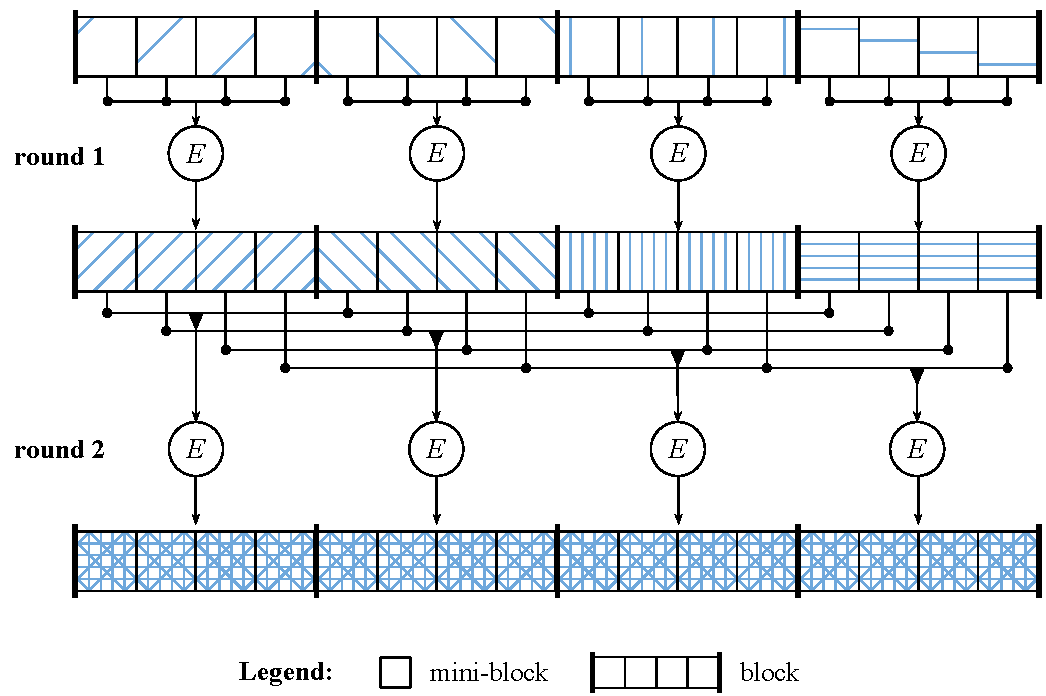
\includegraphics[width=0.8\textwidth]{figures/bdfprs-fig01}
	\end{center}
	\caption{\label{dcs:fig:mixing}An example of application of \name}
\end{figure}



The basic building block enabling the development of our solution is
the application, at the client-side, of an {\em
  All-Or-Nothing-Transform\/} (AONT) encryption mode that transforms
resources for their external storage.  This mode requires the use of
an encryption key. The encryption driven by the key represents the
primary protection, and the use of AONT encryption mode further
strengthens security. An AONT-encryption mode transforms a plaintext
resource (original content in whatever form) into a ciphertext, with
the property that the whole result of the transformation is required
to obtain back the original plaintext. AONT guarantees in fact
complete interdependence ({\em mixing\/}) among the bits of the
encrypted resource in such a way that the unavailability of a portion
of the encrypted resource prevents the reconstruction of any portion
of the original plaintext. A party having access to a portion of the
encrypted resource (but not to the encrypted resource in its
entirety): {\em i)\/} if knowing the encryption key, it will not be able
to reconstruct any portion of the resource (i.e., it will not be able
to derive any information from the AONT-encrypted portions it has; the
only option would be to attempt a brute force attack on the possible
configurations of the missing portions, but their possible large size
makes this attack unfeasible); {\em ii)\/} if not knowing the
encryption key, it will not be able to perform brute-force attacks for
guessing such a key, as any key (even the correct one) will be
ineffective if not applied to the complete resource.  AONT protection
schemes can be built with the use of common cryptographic functions,
like symmetric encryption and hash functions.  An example of AONT
scheme that guarantees complete mixing, which has also been used in
the implementation of our prototype, is
\name~\cite{bdfprs-ccs2016}. Intuitively, \name\ works by applying
different rounds of encryption, each operating on a carefully designed
combination of the bits resulting from the previous round.  With
\name, $i$ rounds of encryption working on blocks including $b$
mini-blocks each, guarantee complete mixing of a resource composed of
$b^i$ mini-blocks.  Figure~\ref{dcs:fig:mixing} illustrates an example of
mixing with two rounds of encryption. The first round mixes contiguous
mini-blocks, while the second round mixes mini-blocks representatives
of the different computations in the first round, providing a mixing
of the whole resource content (as visible from the pattern-coding in
the figure).  \name\ guarantees that each bit in the encrypted
resource depends on the value of each bit in its plaintext
representation.  In our context, the use of AONT guarantees protection
to the individual slices (and shards) composing the resource, and
therefore to the resource itself (in its entirety as well as any of
its portions). In fact, AONT makes each portion of the resource
needed, in terms of information theory, to reconstruct any of the
portions of the resource. The protection is then provided by the
absence of information content.

Figure~\ref{dcs:fig:scenario} illustrates our reference scenario.  The
focus of this chapter is the design of proper {\em slicing\/} of
resources and the {\em allocation\/} of the produced slices to
different nodes in the DCS system.  Note that in the chapter we use the
term {\em slicing\/} to refer to the cutting of a resource and the
term {\em slices\/} to refer to the result of such a process.  A slice
is therefore a chunk of the resource and represents a unit of
allocation, in contrast to a shard that represents a portion of the
resource allocated to a node (a shard can include several slices).
Our approach focuses on {\em slicing\/} and {\em allocation\/} and is
agnostic with respect to the specific AONT technique to be used, as
long as the aimed strong protection guarantees are ensured, and with
respect to the specific DCS adopted.

\begin{figure}
	\begin{center}
		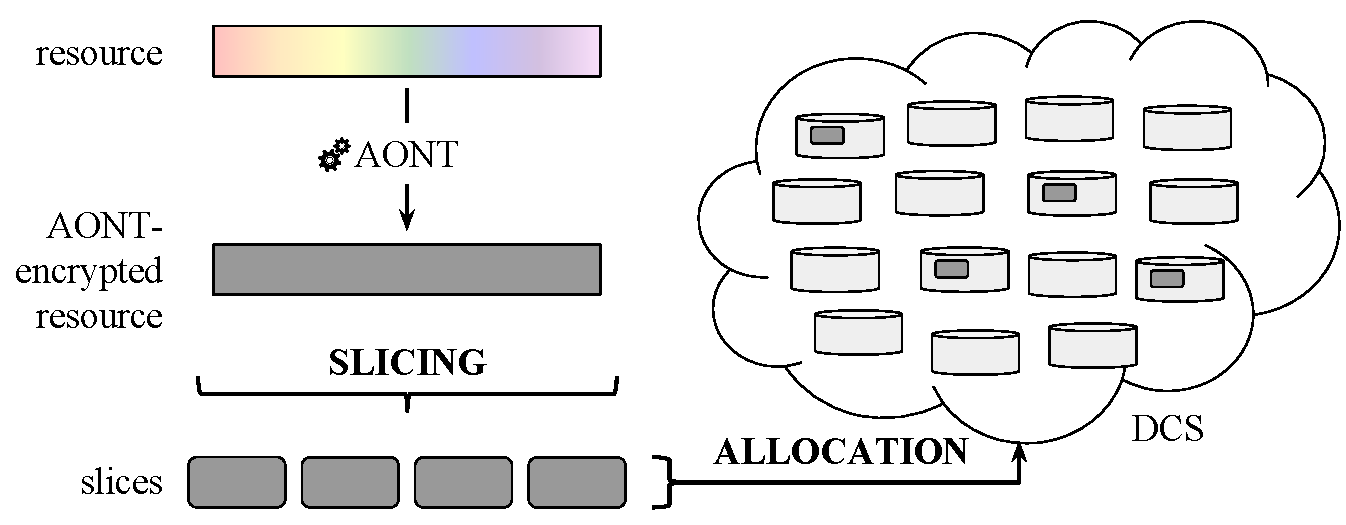
\includegraphics[width=0.9\textwidth]{figures/bdfprs-fig02.pdf}
	\end{center}
	\caption{\label{dcs:fig:scenario}Reference scenario}
\end{figure}




\section{Allocation Properties}\label{dcs:sec:allocation}

In our approach, the slicing of the resources into several slices to
be distributed at the different nodes is guided by the availability
and protection properties that need to be guaranteed.  Availability
(despite nodes failure or temporary unreachability) is provided
through replication, security is provided through protection against
malicious coalitions. Malicious nodes (and coalitions thereof) are
interested in making the resource unavailable, by not returning the
slices of the resource they store, or in providing access to a
resource even after its deletion, by not removing the slices of the
resource they store and returning such slices to (not authorized)
users who pay for it.  Before addressing slicing, we then characterize
the replication and coalition resistance properties of the
distribution of a resource.

We assume a (transformed) resource that has undergone AONT encryption
(as described in the previous section) at the client side. For
simplicity, we will omit such an explicit remark on transformation and
we will simply use the term resource to denote an AONT-encrypted
resource.  Also, we assume a resource to be composed of different
slices, for distribution in a DCS. We will address the problem of
producing such slices in Section~\ref{dcs:sec:functions}.

We model a resource as a set
$\Shards=\{\shard{1},\ldots,\shard{\ns}\}$ of slices to be allocated
to the nodes, denoted \Nodes, of the DCS.  The following definition
formalizes slice allocation.

\smallskip
\begin{definition}[\label{dcs:def:assignment}Allocation function]
Let \Shards\ be a set of slices composing a resource and \Nodes\ be a
set of nodes. An {\em allocation function\/} $\f : \Shards \rightarrow
\Powerset \setminus \emptyset$ assigns each slice $\shard{i} \in
\Shards$ to a set of nodes $\f(\shard{i})=\setnode{i} \subseteq
\Nodes$, $\setnode{i} \neq \emptyset$.
\end{definition}
\smallskip

The allocation function dictates how slices are allocated to nodes in
the DCS. The consideration of sets of nodes (in contrast to individual
nodes) in the co-domain accommodates replication. The exclusion of the
empty set of nodes ensures lossless distribution (i.e., each slice is
allocated to at least one node).  Figure~\ref{dcs:fig:k3_r2} illustrates
an example of an allocation function, considering a resource split
into ten slices ($\Shards=\{\shard{1},\ldots,\shard{10}\}$) allocated
to five nodes ($\node{1},\ldots,\node{5}$) in the DCS (nodes not used
in the allocation are not reported in the figure).  The figure has a
row for each node and a column for each slice. The allocation of a
slice to a node is represented by a gray box at the intersection
between the row representing the node and the column representing the
slice. Empty boxes with a dotted frame represent the fact that the
slice is not allocated to the node.  For example,
$\f(\shard{1})=\{\node{1},\node{2}\}$.


 \begin{figure}[t]
   \begin{center}
     \usetikzlibrary{matrix}
\usetikzlibrary{positioning}

\begin{tikzpicture}
\tikzset{fullnode/.style={fill=black!50}}
\tikzset{emptynode/.append style={densely dotted,draw=black,fill=white}}

\newcommand\CellText[2]{%
	\node[left=of mat#1,anchor=east]
	at ([xshift=5ex]mat#1.west)
	{#2};
}
	
\newcommand\SlText[2]{%
	\node[left=of mat#1,anchor=west]
	at ([yshift=2ex,xshift=3.5ex]mat#1.north)
	{#2};
}


\newcommand{\hhlline}[3]{\draw ([xshift=-4ex,yshift=-0.5ex]#1-#2-1.south west) -- ([yshift=-0.5ex]#1-#2-#3.south east);}
\newcommand{\hupline}[3]{\draw ([xshift=-4ex,yshift=+0.5ex]#1-#2-1.north west) -- ([yshift=+0.5ex]#1-#2-#3.north east);}

\matrix[matrix of nodes,row sep=1ex,column sep=.5ex, nodes={rectangle,draw=black,text width=1ex,align=center,rounded corners=.4ex},text depth=0ex,text height=1ex,nodes in empty cells,baseline=-1ex] (mat1)
{
  |[fullnode]| & |[fullnode]| & |[fullnode]| & |[fullnode]| & |[emptynode]| & |[emptynode]| & |[emptynode]| & |[emptynode]| & |[emptynode]| & |[emptynode]| \\
  |[fullnode]| & |[emptynode]| & |[emptynode]| & |[emptynode]| & |[fullnode]| & |[fullnode]| & |[fullnode]| & |[emptynode]| & |[emptynode]| & |[emptynode]| \\
  |[emptynode]| & |[fullnode]| & |[emptynode]| & |[emptynode]| & |[fullnode]| & |[emptynode]| & |[emptynode]| & |[fullnode]| & |[fullnode]| & |[emptynode]| \\
  |[emptynode]| & |[emptynode]| & |[fullnode]| & |[emptynode]| & |[emptynode]| & |[fullnode]| & |[emptynode]| & |[fullnode]| & |[emptynode]| & |[fullnode]| \\
  |[emptynode]| & |[emptynode]| & |[emptynode]| & |[fullnode]| & |[emptynode]| & |[emptynode]| & |[fullnode]| & |[emptynode]| & |[fullnode]| & |[fullnode]| \\
};

\hupline{mat1}{1}{10}; % first line

\hhlline{mat1}{1}{10};
\hhlline{mat1}{2}{10};
\hhlline{mat1}{3}{10};
\hhlline{mat1}{4}{10};
\hhlline{mat1}{5}{10};

\SlText{1-1-1}{$\tt s_{1}$}
\SlText{1-1-2}{$\tt s_{2}$}
\SlText{1-1-3}{$\tt s_{3}$}
\SlText{1-1-4}{$\tt s_{4}$}
\SlText{1-1-5}{$\tt s_{5}$}
\SlText{1-1-6}{$\tt s_{6}$}
\SlText{1-1-7}{$\tt s_{7}$}
\SlText{1-1-8}{$\tt s_{8}$}
\SlText{1-1-9}{$\tt s_{9}$}
\SlText{1-1-10}{$\tt s_{10}$}
		
\CellText{1-1-1}{$\tt n_{1}$};
\CellText{1-2-1}{$\tt n_{2}$};
\CellText{1-3-1}{$\tt n_{3}$};
\CellText{1-4-1}{$\tt n_{4}$};
\CellText{1-5-1}{$\tt n_{5}$};

\end{tikzpicture}
 \end{center}
 \caption{An example of a minimal 3-protected and 2-replicated allocation function}
 \label{dcs:fig:k3_r2}
 \end{figure}


We identify two main properties of an allocation, characterizing the
availability, provided by {\em replication}, and the {\em protection}
against possible malicious coalitions of nodes, provided by the
diversification of the allocation.

We characterize availability provided by replication in terms of the
number of replicas maintained in the system. While in principle the
number of replicas maintained for each slice can differ, we assume the
same number of replicas is used for all the slices. This derives from
the fact that we assume that nodes are not associated with individual
reliability profiles (Section~\ref{dcs:sec:analysis}).  Since all slices
are needed to reconstruct the resource, using fewer replicas for any
of the slices would decrease the availability of the resource, which
will be dictated by such a lower bound.  The following definition
formalizes the replication degree of an allocation function.

\smallskip
\begin{definition}[\label{dcs:def:replicated}\texorpdfstring{$\boldsymbol{\nr}$}{r}-Replicated allocation function]
Let \Shards\ be a set of slices composing a resource, \Nodes\ be a set
of nodes, and \f\ be an allocation function. Function \f\ is {\em
  \nr-replicated} iff $\forall \shard{i}\in\Shards$, $|\f(\shard{i})|
\geq \nr$.
\end{definition}
\smallskip

For instance, the allocation function in Figure~\ref{dcs:fig:k3_r2} is
2-replicated, as two copies are maintained for each slice.

We characterize the protection offered by an allocation in terms of
the minimum number of nodes required to reconstruct a resource, as
formalized by the following definition.

\smallskip
\begin{definition}[\label{dcs:def:protected}\texorpdfstring{$\boldsymbol{\nk}$}{k}-Protected allocation function]
Let \Shards\ be a set of slices composing a resource, \Nodes\ be a set
of nodes, and \f\ be an allocation function. Function \f\ is {\em
  \nk-protected} iff for each $\setnode{i} \subset \Nodes$, with
$|\setnode{i}| \leq \nk$, $\exists \shard{j} \in \Shards$
s.t. $\f(\shard{j})\cap\setnode{i}=\emptyset$.
\end{definition}
\smallskip

A \nk-protected allocation function guarantees distribution of slices
to nodes in such a way to dictate the cooperation of no less than
$\nk+1$ nodes to collect all the slices composing the resource (and
hence enabling retrieving its plaintext). In other words, a
\nk-protected allocation function guarantees protection of the
resource against malicious (i.e., colluding) behavior of up to
\nk\ nodes. In fact, with a \K-protected allocation function, for each
coalition of \K\ nodes in \Nodes, there is at least a slice that is
not stored at any of the nodes in the coalition. Hence, such a
coalition can neither decrypt the resource with a brute-force attack,
nor prevent its deletion. The allocation function in
Figure~\ref{dcs:fig:k3_r2} is 3-protected: any subset of $3$ out of the
$5$ nodes misses at least a slice.  For instance, coalition
\{\node{1},\node{2},\node{3}\} misses slice \shard{10}, while
coalition \{\node{1},\node{2},\node{4}\} misses slice \shard{9}. On
the contrary, the allocation function in Figure~\ref{dcs:fig:k2_r2}, on
the same slices and nodes, is not 3-protected (but only 2-protected):
coalition \{\node{1},\node{3},\node{4}\} jointly possesses all the
slices.

\begin{figure}[t]
  \begin{center}
    \usetikzlibrary{matrix}
\usetikzlibrary{positioning}

\begin{tikzpicture}
\tikzset{fullnode/.style={fill=black!50}}
\tikzset{emptynode/.append style={densely dotted,draw=black,fill=white}}

\newcommand\CellText[2]{%
	\node[left=of mat#1,anchor=east]
	at ([xshift=5ex]mat#1.west)
	{#2};
}
	
\newcommand\SlText[2]{%
	\node[left=of mat#1,anchor=west]
	at ([yshift=2ex,xshift=3.5ex]mat#1.north)
	{#2};
}


\newcommand{\hhlline}[3]{\draw ([xshift=-4ex,yshift=-0.5ex]#1-#2-1.south west) -- ([yshift=-0.5ex]#1-#2-#3.south east);}
\newcommand{\hupline}[3]{\draw ([xshift=-4ex,yshift=+0.5ex]#1-#2-1.north west) -- ([yshift=+0.5ex]#1-#2-#3.north east);}

\matrix[matrix of nodes,row sep=1ex,column sep=.5ex, nodes={rectangle,draw=black,text width=1ex,align=center,rounded corners=.4ex},text depth=0ex,text height=1ex,nodes in empty cells,baseline=-1ex] (mat1)
{
  |[fullnode]| & |[fullnode]| & |[fullnode]| & |[fullnode]| & |[emptynode]| & |[emptynode]| & |[emptynode]| & |[emptynode]| & |[emptynode]| & |[emptynode]| \\
  |[fullnode]| & |[fullnode]| & |[fullnode]| & |[emptynode]| & |[fullnode]| & |[emptynode]| & |[emptynode]| & |[emptynode]| & |[emptynode]| & |[emptynode]| \\
  |[emptynode]| & |[emptynode]| & |[emptynode]| & |[fullnode]| & |[fullnode]| & |[fullnode]| & |[fullnode]| & |[emptynode]| & |[emptynode]| & |[emptynode]| \\
  |[emptynode]| & |[emptynode]| & |[emptynode]| & |[emptynode]| & |[emptynode]| & |[fullnode]| & |[emptynode]| & |[fullnode]| & |[fullnode]| & |[fullnode]| \\
  |[emptynode]| & |[emptynode]| & |[emptynode]| & |[emptynode]| & |[emptynode]| & |[emptynode]| & |[fullnode]| & |[fullnode]| & |[fullnode]| & |[fullnode]| \\
};

\hupline{mat1}{1}{10}; % first line

\hhlline{mat1}{1}{10};
\hhlline{mat1}{2}{10};
\hhlline{mat1}{3}{10};
\hhlline{mat1}{4}{10};
\hhlline{mat1}{5}{10};

\SlText{1-1-1}{$\tt s_{1}$}
\SlText{1-1-2}{$\tt s_{2}$}
\SlText{1-1-3}{$\tt s_{3}$}
\SlText{1-1-4}{$\tt s_{4}$}
\SlText{1-1-5}{$\tt s_{5}$}
\SlText{1-1-6}{$\tt s_{6}$}
\SlText{1-1-7}{$\tt s_{7}$}
\SlText{1-1-8}{$\tt s_{8}$}
\SlText{1-1-9}{$\tt s_{9}$}
\SlText{1-1-10}{$\tt s_{10}$}
		
\CellText{1-1-1}{$\tt n_{1}$};
\CellText{1-2-1}{$\tt n_{2}$};
\CellText{1-3-1}{$\tt n_{3}$};
\CellText{1-4-1}{$\tt n_{4}$};
\CellText{1-5-1}{$\tt n_{5}$};

\end{tikzpicture}
 \end{center}
\caption{An example of 2-replicated allocation function that is not 3-protected}
\label{dcs:fig:k2_r2}
\end{figure}

We refer to an allocation function that is \nr-replicated, according
to Definition~\ref{dcs:def:replicated}, and \nk-protected, according to
Definition~\ref{dcs:def:protected}, as a {\em $(\nk,\nr)$-allocation\/}.

\smallskip
\begin{definition}[\label{dcs:def:krallocation}$(\nk,\nr)$-Allocation]
Let \Shards\ be a set of slices composing a resource, \Nodes\ be a set
of nodes, and \f\ be an allocation function. Function \f\ is a {\em
  $(\nk,\nr)$-allocation} iff it is {\em \nk-protected} and {\em
  \nr-replicated}.
\end{definition}
\smallskip

According to Definitions~\ref{dcs:def:replicated} and~\ref{dcs:def:protected},
a $(\nk,\nr)$-allocation is also a $(\nk',\nr')$-allocation, for any
$\nr'\leq\nr$ and any $\nk'\leq\nk$. In fact, trivially, an allocation
function providing $\nr$ replicas also provides $\nr'<\nr$
replicas. Analogously, an allocation function protecting a resource
from coalitions of \nk\ nodes also protects the resource from
coalitions of $\nk'<\nk$ nodes. Among all $(\nk,\nr)$-allocations, we
are interested in identifying those for which \nk\ and \nr\ represent
the highest values satisfying the availability and protection
properties (i.e.,  satisfying the
properties in a minimal way). We call such allocation functions
minimal, as formalized by the following definition.

\smallskip
\begin{definition}[\label{dcs:def:minimal}Minimal $(\nk,\nr)$-allocation]
Let \Shards\ be a set of slices composing a resource, \Nodes\ be a set of nodes, 
and \f\ be a $(\nk,\nr)$-allocation. Function \f\ is  {\em minimal\/} 
iff:
\begin{align*} 
    & \text{1. }\ \text{it is not } (\nk+1)\text{-protected}\ ; \\
    & \text{1. }\ \forall \shard{i} \in \Shards \text{ , } |\f(\shard{i})| = \nr\ .
\end{align*}
\end{definition}

\smallskip

According to Definition~\ref{dcs:def:minimal}, a {\em minimal\/}
$(\nk,\nr)$-allocation is an allocation that guarantees protection
against coalitions of up to $k$ (but no more) nodes and that uses
exactly $r$ replicas.  The allocation function in
Figure~\ref{dcs:fig:k3_r2} is an example of minimal $(3,2)$-allocation.
In the following, we will restrict our attention to minimal allocation
functions and, when talking about a $(\nk,\nr)$-allocation, we will
implicitly assume such minimality.




\section[Strategies]{Slicing and Allocation Strategies}\label{dcs:sec:functions}

In the absence of replication, producing an allocation that guarantees
$\nk$-protection, that is, a $(\nk,1)$-allocation, is straightforward:
it is sufficient to split the resource into $\nk+1$ slices and
allocate each slice to a different node.  When considering
replication, different approaches can be taken for allocation,
differing in the granularity of slicing and in how allocation
diversifies the storage at different nodes.  In the following, we
discuss these options. In the discussion, in addition to parameters
$\nk$ and $\nr$ introduced before, we will use parameters $\ns$,
denoting the number of slices in which a resource is split, and $\nn$,
denoting the number of nodes to be involved in the allocation of a
resource.  Different approaches vary in the number $\ns$ of slices to
be considered and in the number $\nn$ of nodes to be involved for
providing a $(\nk,\nr)$-allocation.  We note that, with respect to
nodes, the only parameter to be considered in the allocation
strategies is the number $\nn$ of nodes to be involved (the specific
nodes to be involved can be selected randomly).  We identify and study
the behavior of two approaches for producing a $(\nk,\nr)$-allocation.
The first approach aims to minimize the number of slices (\Diagonal),
while the second aims to minimize the number of nodes (\Compact). We
analyze these two approaches as they represent the two extremes with
respect to granularity of slicing and diversification of
allocation. Their analysis permits to highlight the characteristics of
fine-grained (\Compact) and coarse-grained (\Diagonal) slicing, and
can also represent a reference for intermediate configurations.


\subsection{Minimizing the number of slices}\label{dcs:ss:diagonal}
 

We start noting that the number $\ns$ of slices involved for
guaranteeing a $(\nk,\nr)$-allocation must be such that $\ns \geq \nk
+1$. In fact, there should be at least $\nk+1$ slices to guarantee
\nk-protection, as formally captured by the following theorem.


\smallskip
\begin{theorem}[\label{dcs:theo:minslices}Minimum number of slices]
Let \nk\ be a protection parameter and \nr\ be a replication
factor. The number \ns\ of slices necessary to define a
$(\nk,\nr)$-allocation is $\ns \geq \nk+1$.
\end{theorem}
\smallskip


A simple approach for determining a $(\nk,\nr)$-allocation extends the
natural approach of producing $\nk+1$ slices, by simply considering
their replication at different nodes.  Such an approach is
characterized by a {\em coarse-slicing\/}, since minimizing the number
of slices clearly entails a larger size for them, and by {\em
  consistent replication} (i.e., nodes have no intersection or
complete intersection of stored slices).

We observe that a $(\nk,\nr)$-allocation function using the minimum
number ($\ns=\nk+1$) of slices implies that:

\begin{enumerate}
	\item a node maintains at most one slice, that is, 
	$|\f^{-1}(\node{i})|=1$, $\forall \node{i} \in \Nodes$ involved in the allocation;
	
	\item the number of nodes involved in the allocation is exactly 
	\nr\ times the number of slices, that is, $\nn=\nr \cdot (\nk+1)$.
\end{enumerate}

The first observation derives from the fact that, since there are only
$\nk+1$ slices, placing more than one slice on a node would imply the
existence of a set of $\nk$ nodes able to reconstruct the resource and
therefore would not guarantee \nk-protection anymore.  The second
observation naturally derives from the first, considering that every
slice needs to be replicated \nr\ times.  The following theorem proves
the observations above.

\smallskip
\begin{theorem}\label{dcs:theo:diagonal}
Let \nk\ be a protection parameter and \nr\ be a replication factor. A
$(\nk,\nr)$-allocation $\f : \Shards \rightarrow \Powerset \setminus
\emptyset$ that adopts the minimum number of slices $\ns=\nk+1$ is
such that:
\begin{align*}
    & \text{1. }\ |\f^{-1}(\node{i})|=1 \text{ , } \forall \node{i} \in \Nodes\ \text{ involved in the allocation}\ ; \\
    & \text{2. }\ \text{the number of nodes involved in the allocation is }\ \nn=\nr \cdot (\nk+1)\ . 
\end{align*}
\end{theorem}
\smallskip


\begin{figure}[t]
  \begin{center}
    \usetikzlibrary{matrix}
\usetikzlibrary{positioning}

\begin{tikzpicture}
\tikzset{fullnode/.style={fill=black!50}}
\tikzset{emptynode/.append style={densely dotted,draw=black,fill=white}}

\newcommand\CellText[2]{%
	\node[left=of mat#1,anchor=east]
	at ([xshift=5ex]mat#1.west)
	{#2};
}
	
\newcommand\SlText[2]{%
	\node[left=of mat#1,anchor=west]
	at ([yshift=2ex,xshift=3.5ex]mat#1.north)
	{#2};
}


\newcommand{\hhlline}[3]{\draw ([xshift=-4ex,yshift=-0.5ex]#1-#2-1.south west) -- ([yshift=-0.5ex]#1-#2-#3.south east);}
\newcommand{\hupline}[3]{\draw ([xshift=-4ex,yshift=+0.5ex]#1-#2-1.north west) -- ([yshift=+0.5ex]#1-#2-#3.north east);}

\matrix[matrix of nodes,row sep=1ex,column sep=.5ex,nodes={rectangle,draw=black,minimum width=6.25ex,align=center,rounded corners=.4ex},text depth=0ex,text height=1ex,nodes in empty cells,baseline=-1ex] (mat1)
{
  |[fullnode]| & |[emptynode]| & |[emptynode]| & |[emptynode]| \\
  |[fullnode]| & |[emptynode]| & |[emptynode]| & |[emptynode]| \\
  |[emptynode]| & |[fullnode]| & |[emptynode]| & |[emptynode]| \\
  |[emptynode]| & |[fullnode]| & |[emptynode]| & |[emptynode]| \\
  |[emptynode]| & |[emptynode]| & |[fullnode]| & |[emptynode]| \\
  |[emptynode]| & |[emptynode]| & |[fullnode]| & |[emptynode]| \\
  |[emptynode]| & |[emptynode]| & |[emptynode]| & |[fullnode]| \\
  |[emptynode]| & |[emptynode]| & |[emptynode]| & |[fullnode]| \\
};

\hupline{mat1}{1}{4}; 

\hhlline{mat1}{1}{4};
\hhlline{mat1}{2}{4};
\hhlline{mat1}{3}{4};
\hhlline{mat1}{4}{4};
\hhlline{mat1}{5}{4};
\hhlline{mat1}{6}{4};
\hhlline{mat1}{7}{4};
\hhlline{mat1}{8}{4};

\SlText{1-1-1}{$\tt s_{1}$}
\SlText{1-1-2}{$\tt s_{2}$}
\SlText{1-1-3}{$\tt s_{3}$}
\SlText{1-1-4}{$\tt s_{4}$}
		
\CellText{1-1-1}{$\tt n_{1}$};
\CellText{1-2-1}{$\tt n_{2}$};
\CellText{1-3-1}{$\tt n_{3}$};
\CellText{1-4-1}{$\tt n_{4}$};
\CellText{1-5-1}{$\tt n_{5}$};
\CellText{1-6-1}{$\tt n_{6}$};
\CellText{1-7-1}{$\tt n_{7}$};
\CellText{1-8-1}{$\tt n_{8}$};


\end{tikzpicture}
 \end{center}
	\caption{An examples of $(3,2)$-allocation that minimizes the number of slices}
	\label{dcs:fig:diagonalese}
\end{figure}

As an example, a $(3,2)$-allocation using the minimum number of slices
would imply splitting the resources into $4$ ($=3+1$) slices,
generating $2$ copies of each slice, to be distributed at 8 different
nodes. Figure~\ref{dcs:fig:diagonalese} illustrates an example of
allocation function enforcing this.


A $(\nk,\nr)$-allocation that uses the minimum number of slices
$\ns=\nk+1$ well resists to failures. Indeed, $\nk+1$ nodes out of
$\nr\cdot(\nk+1)$ are sufficient to reconstruct the resource content,
as long as one replica of each slice is available. However, the number
of nodes used by such an allocation function quickly grows with
\nk\ and \nr. For instance, a $(10,5)$-allocation would need 55
$(=5\cdot(10+1))$ nodes.


\subsection{Minimizing the number of nodes}\label{dcs:ss:kompact}

At the other end of the spectrum of possible strategies for
defining and distributing slices to guarantee a $(\nk,\nr)$-allocation,
there are functions minimizing the number of nodes to be involved in the distribution
(and deriving the number of slices in which the
resource needs to be split based on this).

A trivial lower bound on the number of nodes that need to be involved
in a $(\nk,\nr)$-allocation is $\nn \geq max(\nk+1,\nr)$, since there
should be at least \nr\ nodes to hold \nr\ replicas and at least
$\nk+1$ nodes to guarantee \nk-protection.  The minimum number of
nodes to be involved to guarantee $(\nk,\nr)$-allocation is actually
higher than that as it needs to be at least the sum of the protection
and replication parameters (\nk\ and \nr), as stated by the following
theorem.

\smallskip
\begin{theorem}[\label{dcs:theo:numnodes}Minimum number of nodes]
Let \nk\ be a protection parameter and \nr\ be a replication
factor. The number \nn\ of nodes necessary to define a
$(\nk,\nr)$-allocation is $\nn \geq \nk+\nr$.
\end{theorem}
\smallskip

The minimum number of nodes stated by Theorem~\ref{dcs:theo:numnodes}
derives from two simple observations. First, to guarantee
\nk-protection, for each coalition of \nk\ nodes, there must exist at
least one slice that is not stored at any of the nodes in the
coalition. Second, to provide \nr-replication, such a slice should be
stored at (at least) \nr\ nodes that are not in the coalition. Hence,
at least $\nk + \nr$ nodes need to be involved. As we will illustrate
in the following, $\nk+\nr$ nodes, besides been necessary, are also
sufficient to define a $(\nk,\nr)$-allocation.

  
While using the minimum number of slices applies a coarse slicing with
consistent replication, using the minimum number of nodes applies a
{\em fine-grained slicing} with {\em diversified replication} across
nodes. Intuitively, instead of splitting the resource into slices and
allocating to each node a single slice, minimizing the number of nodes
requires slicing the resource into more fine-grained slices and
allocating the slices to nodes in a diversified manner, to guarantee
that no set of \nk\ nodes jointly possesses all the slices.  The
definition of the allocation requires then to identify the number of
slices in which a resource needs to be split, which must be sufficient
to distribute the \nr\ replicas to nodes while ensuring
\nk-protection. The minimum number of slices needed for ensuring that
no set of \nk\ nodes is able to reconstruct the resource when using
$\nk+\nr$ nodes, clearly happens when any set of \nk\ nodes misses
exactly one slice (which, given \nr-replication, would instead be
stored at the \nr\ nodes not belonging to the set) and no two
coalitions miss the same slice. In fact, if two sets of \nk\ nodes
miss the same slice, such a slice could not have \nr\ replicas when
using only $\nk+\nr$ nodes. The number of required slices can then be
identified as the number of coalitions of \nk\ nodes out of $\nk+\nr$,
that is $\binom{\nk+\nr}{\nk}$, as formally proved by the following
theorem.


\smallskip
\begin{theorem}\label{dcs:theo:numslices}
Let \nk\ be a protection parameter and \nr\ be a replication
factor. Each $(\nk,\nr)$-allocation that adopts the minimum number of
nodes $\nn = \nk+\nr$ uses $\ns=\binom{\nn}{\nk}=\binom{\nk+\nr}{\nk}$
slices.
\end{theorem}
\smallskip

A $(\nk,\nr)$-allocation that uses $\nk+\nr$ nodes and
$\binom{\nk+\nr}{\nk}$ slices has two interesting properties. The
first one, already noted, is that any coalition of \nk\ nodes {\em
  misses exactly one} slice. The second one, deriving from the fact
that the missing slice is different for different coalitions, is that
{\em any\/} set of $\nk+1$ nodes is sufficient to reconstruct the
resource (differently from the \Diagonal\ approach where at least
$\nk+1$ nodes are needed to reconstruct the resource but not any set
of $\nk+1$ nodes guarantees that). The following theorem proves these
two properties.



\smallskip
\begin{theorem}\label{dcs:theo:p4}
Let \nk\ be a protection parameter and \nr\ be a replication
factor. Each $(\nk,\nr)$-allocation that adopts the minimum number of
nodes $\nn = \nk+\nr$ and $\ns=\binom{\nk+\nr}{\nk}$ slices guarantees
that:
	\begin{align*}
	    & \text{1. }\ \forall \setnode{i} \subset \Nodes \text{ with } |\setnode{i}| = \nk \text{, } \nexists\  \shard{j} \text{ s.t. } \f(\shard{j})\cap\setnode{i}=\emptyset\ ; \\
	    & \text{2. }\ \forall \setnode{i} \subseteq \Nodes \text{ with } |\setnode{i}| = \nk+1 \text{, } \bigcup_{\node{j}\in\setnode{i}} \f^{-1}(\node{j}) = \Shards\ .
	\end{align*}
\end{theorem}
\smallskip



A $(\nk,\nr)$-allocation that minimizes the number of nodes can be
obtained by assuming \Nodes\ to comprise $\nk + \nr$ nodes and
proceeding as follows. Let $\Powersetk = \{\setnode{i}\in\Powerset :
|\setnode{i}|=\nk\}$ be all subsets of \nk\ nodes in \Nodes. For each
slice $\shard{i}\in\Shards, i=1,\ldots,\binom{\nk+\nr}{\nk}$,
$\f(\shard{i})=\{\Nodes\ \setminus \{\setnode{i}\}:$ with
\setnode{i}$\in$$\Powersetk$\}.  Intuitively, for each slice
\shard{i}, \f(\shard{i}) selects a coalition of \nk\ nodes that misses
\shard{i} and allocates slice \shard{i} to all the other nodes. This
guarantees that each coalition (\setnode{i}) of \nk\ nodes misses at
least one slice (\shard{i}), providing \nk-protection. Slice
\shard{i}, which represents the missing slice for coalition
\setnode{i}, is stored at all the other $\nn-\nk=\nr$ nodes in \Nodes,
providing \nr-replication.  Intuitively, in a $(\nk,\nr)$-allocation
using the minimum number of nodes, no two slices are allocated exactly
to the same set of nodes (i.e., $\forall \shard{i},\shard{j} \in
\Shards$, \f(\shard{i})$\neq$\f(\shard{j})).  In fact, the possible
subsets of \nr\ nodes in \Nodes\ is $\binom{\nk+\nr}{\nr}$ and
$\binom{\nk+\nr}{\nk}=\binom{\nk+\nr}{\nr}$.

For example, a $(3,2)$-allocation using the minimum number of nodes
requires $\nn=\nk+\nr=3+2=5$ nodes and the use of 
$\ns=\binom{\nk+\nr}{\nk}=\binom{5}{3}=10$ slices. Figure~\ref{dcs:fig:k3_r2} 
illustrates an example of $(3,2)$-allocation distributing 10 slices over 
 $5$ nodes. 
The allocation is a $(3,2)$-allocation since it replicates each slice twice 
while guaranteeing that no coalition of $3$ nodes possesses all the slices.
More precisely, any coalition of $3$ nodes misses exactly one slice
and the missing slice is different for any of such coalitions.
For instance, coalition $\{\node{1},\node{2},\node{3}\}$ 
misses slice \shard{10}, while coalition $\{\node{1},\node{2},\node{4}\}$
misses slice \shard{9}. 



\subsection{Discussion}
We have discussed two alternative strategies for producing a
$(\nk,\nr)$-allocation, aimed to minimize the number of slices (
  \diagonal, with coarse-grained slicing and consistent
replication) and to minimize the number of involved nodes (\compact
    , with fine-grained slicing and diversified
  replication).  When no replication is used (i.e., $\nr=1$) these two
  strategies are equivalent, as each would imply the use of the same
  number of slices $\ns=k+1$ and nodes $\nn=k+1$. On the contrary,
  when replication is adopted (i.e., $\nr>1$) the two strategies
  differ in the number of nodes \nn\ and slices \ns\ used and in the
  distribution of slices to nodes. Besides these two extreme
  configurations, the resource owner can decide to adopt other
  allocation strategies. The analysis presented in this section can
  then represent a reference for the definition and analysis of
  intermediate configurations.

We note that the structure of the \compact strategy has a
correspondence with {\em secret sharing}~\cite{shamir1979share}. In
($m$,$d$) secret sharing, the goal is to build $d$ shares of a secret
such that at least $m$ of them are necessary to reconstruct a
secret. Given a \compact $(\nk,\nr)$-allocation, with
$\nk+\nr$ shares, the use of a ($\K+1$, $\K+\nr$) secret sharing
scheme would then satisfy the requirement that at least $\K+1$ nodes
have to cooperate to access the resource, tolerating the loss of up to
$\R-1$ nodes. Compared to the well-known Shamir's technique for secret
sharing~\cite{shamir1979share}, the approach we propose shows a
significant advantage with respect to storage and network capacity. In
terms of computational cost, Shamir's technique requires to identify
the roots of a polynomial, while our approach requires the application
of symmetric encryption algorithms. The performance of symmetric
encryption algorithms is so high, particularly for algorithms
implemented in hardware by the CPU, that the potentially simpler
computational structure of Shamir's technique does not provide an
advantage and turns out to be slower when considering large
resources. However, the computational cost is in any case a marginal
element in this domain. In terms of storage, Shamir's approach offers
security if each of the shares has the same size as the secret. With a
($\K+1$, $\K+\nr$) secret sharing scheme, there is therefore the need
to store in the network $\K+\R$ times the amount of plaintext data,
whereas our solution is characterized by the replication factor \R.
In terms of the minimum amount of data that has to be accessed by the
owner, Shamir's solution asks the owner to read $\K+1$ times the size
of the plaintext, whereas our technique, if the storage nodes support
access to portions of the resource, does not require to access more
than the size of the plaintext.  We can then conclude that Shamir's
technique, which is quite interesting for domains where the secret has
a small size (e.g., encryption keys), is not convenient in the domain
considered in this work. When Shamir's method is used to protect only
the encryption key and then encryption is used to protect the
resource, Shamir's method can be assumed to be only a key management
strategy, making encryption of the resource the only protection
measure, without offering the level of protection provided by AONT.

Note also that, for simplicity, we have assumed that the owner can
arbitrarily split her resource as needed for the definition of a
$(\nk,\nr)$-allocation. However, thanks to its flexibility, our
approach can be adopted also when the encrypted resource is already
organized in {\em chunks} that cannot be split for allocation (e.g.,
blocks resulting from the AONT algorithm adopted), or in general when
slicing is constrained. Indeed, even if in the discussion, for
simplicity, we consider slices of equal size, our approach can be
adopted also if the size varies.  Also, slices can contain
non-contiguous chunks of the resource. Clearly, the number of chunks
should be sufficient for the definition of a $(\nk,\nr)$-allocation
(e.g., $\nk+1$ and $\binom{\nn}{\nk}$ in our two alternative
configurations). If the resource includes fewer chunks, it needs to be
padded. If the resource includes more chunks than necessary, the
resource owner can combine the chunks in \ns\ slices and apply the
chosen allocation function over these slices. As an example, to define
a (3,2)-allocation for a resource organized in 20 chunks using 5
nodes, chunks can be arbitrarily combined to identify 10 slices for
allocation. Alternatively, \nk-protection and \nr-replication can be
obtained by considering each chunk as a different slice and
interpreting the allocation function as periodic in \ns, or simply by
randomly allocating the chunks after the first \ns\ (which are the
ones necessary to guarantee \nk-protection). For instance, a
(3,2)-allocation for a resource with 20 chunks using 5 nodes can be
obtained by applying the allocation function in Figure~\ref{dcs:fig:k3_r2}
twice (on slices $\shard{1},\ldots,\shard{10}$ and
$\shard{11},\ldots,\shard{20}$), or by using it for slices
$\shard{1},\ldots,\shard{10}$ while arbitrarily allocating slices
$\shard{11},\ldots,\shard{20}$ at two nodes each.


\section[Guarantees]{Availability and Protection Guarantees}\label{dcs:sec:analysis}

Parameters \nr\ and \nk\ introduced in the previous section
characterize the degree of replication and of protection against
malicious coalitions of nodes.  Such parameters provide a clean and
precise modeling and allow reasoning about properly setting the number
of slices and the number of nodes to be involved in the allocation.
The setting of \nk\ and \nr\ to provide given security and
availability guarantees clearly depends on the specific
characteristics of the network.  For instance, in a stable network a
low number of replicas may suffice to provide high availability, while
in a highly dynamic and non-resilient network a higher number of
replicas should be used to enjoy the same guarantee. In the same vein,
actual protection against possible exposure of a resource to malicious
coalitions depends on the nature of nodes involved in the allocation.
Consistently with these observations, we note that a natural way for
the resource owner to express and reason about availability and
protection guarantees is the probability of the resource to become
unavailable and the probability of a coalition of malicious nodes to
jointly possess all the resource slices.  In this section, we
illustrate how to derive proper \nr\ and \nk\ settings to be then used
for splitting resources into slices and for slices allocation,
starting from the aimed guarantee of availability and security
expressed in terms of such probabilities.  Clearly, the probability of
a resource to become unavailable, or exposed to malicious coalitions,
depends on the probability of individual nodes to become unavailable
or behaving maliciously.  We then introduce the probability of a
single node to fail, and hence to become unavailable, denoted \pf, and
the probability of a node to behave maliciously, and hence to
participate in a malicious coalition compromising protection, denoted
\pc.  We assume, as common in decentralized systems, the probability
\pf\ of failure to be the same for all nodes and the failure of any
node to be not influenced by the failure of the other nodes. This
assumption enables a clean modeling, which can be taken as a reference
for reasoning on different probability distributions. Since the
selection of storage nodes is driven by a pseudorandom function, we
also consider a uniform probability \pc\ of compromise and assume
independence of compromise events on different nodes.  We introduce
the probability of a resource to become unavailable, denoted $\PF$,
and of being exposed to a malicious coalition, denoted $\PC$, when
using a $(\nk,\nr)$-allocation.  The analysis will then guide the
identification of the values for \nk\ and \nr\ to be used to guarantee
that $\PF$ and $\PC$ do not exceed a given threshold.  We discuss
separately the \diagonal\ and \compact\ allocation strategies
introduced in the previous section, which, as we will see, exhibit a
different behavior with respect to availability and security
guarantees.

\begin{figure}[t]
	\centering
	\hspace*{-25pt}
	\setlength{\tabcolsep}{20pt}
	\begin{tabular}{cccc}
	    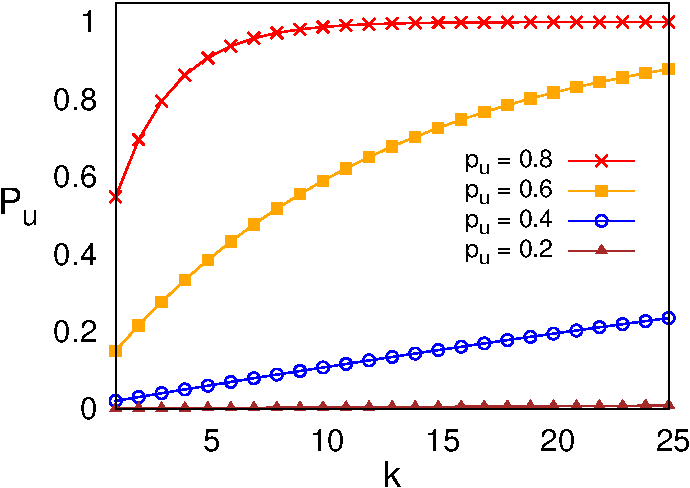
\includegraphics[width=0.45\textwidth]{figures/bdfprs-fig06a} &
	    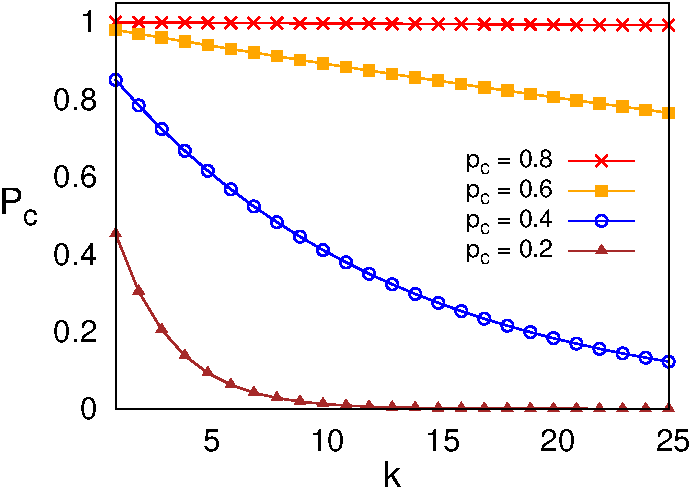
\includegraphics[width=0.45\textwidth]{figures/bdfprs-fig06b} \\[3pt]
	    \footnotesize{\hspace{20pt}(a) $\nk=1,\ldots,25$, $\nr=5$} &
	    \footnotesize{\hspace{20pt}(b) $\nk=1,\ldots,25$, $\nr=5$} \\[20pt]
	    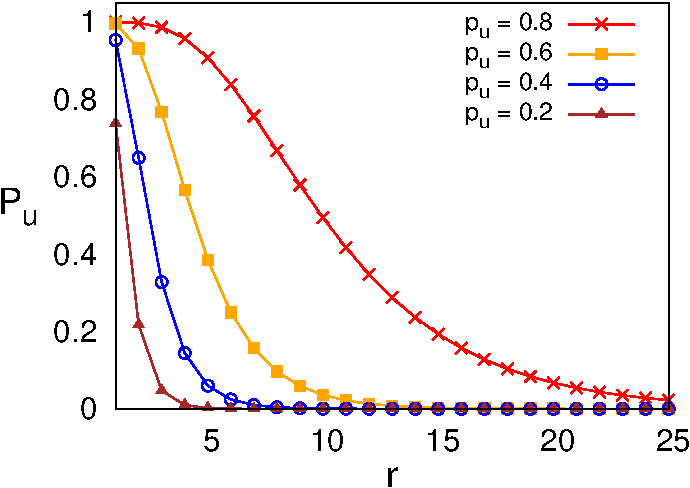
\includegraphics[width=0.45\textwidth]{figures/bdfprs-fig06c} &
	    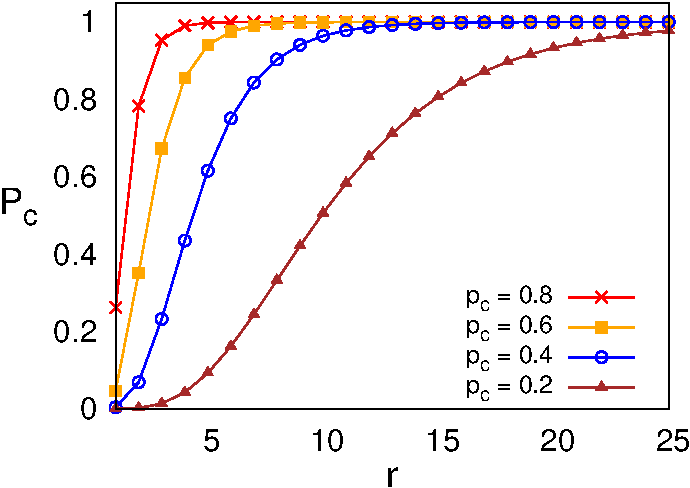
\includegraphics[width=0.45\textwidth]{figures/bdfprs-fig06d} \\[3pt]
	    \footnotesize{\hspace{20pt}(c) $\nk=5$, $\nr=1,\ldots,25$} & 
	    \footnotesize{\hspace{20pt}(d) $\nk=5$, $\nr=1,\ldots,25$} \\[20pt]
	\end{tabular}
    \caption{\label{dcs:fig:diagonal} Probability that the resource is unavailable (a,c) and that it is exposed (b,d) using a $(\nk,\nr)$-allocation that minimizes the number of slices, with \nr=5 varying \nk\ between 1 and 25 (a,b), and with \nk=5 varying \nr\ between 1 and 25 (c,d)}
\end{figure}

\subsection{\diagonal allocation}\label{dcs:sec:minslice}
Using a $(\nk,\nr)$-allocation with the minimum number of slices,
unavailability of a resource happens when, for any of the $\nk+1$
slices composing the resources, all the \nr\ nodes storing the replica
of the slice fail. The probability of such an event to happen is $\PF=
1 - (1-(\pf)^{\R})^{\K+1}$, where $(1-(\pf)^{\R})$ is the probability
that one of the \nr\ replicas of a slice is available and, for the
assumption on the independence of the failure events,
$(1-(\pf)^{\R})^{\K+1}$ is the probability that one replica of each of
the $\nk+1$ slices is available. In the same vein, the resource
becomes exposed (and hence a compromise happens and deletion cannot be
guaranteed) when a coalition of malicious nodes collectively possesses
all the $\nk+1$ slices, that is, when the coalition contains $\nk+1$
nodes each possessing a different slice. The probability of such an
event to happen is $\PC= (1 - (1-\pc)^{\R})^{\K+1}$, where
$(1-\pc)^{\R}$ is the probability that one replica is stored on a node
that is not part of a coalition and, consequently, $1-(1-\pc)^{\R}$ is
the probability that one replica is exposed. Since such an exposure
must involve all the $\nk+1$ slices, the probability that a coalition
possesses all the slices is $(1 - (1-\pc)^{\R})^{\K+1}$. The following
theorem proves such observations.

\smallskip
\begin{theorem}\label{dcs:teo:probability-diagonal}
Given a set \Shards\ of slices composing a resource, a set \Nodes\ of nodes with probability of failure \pf\ and probability of being compromised \pc, and a $(\nk,\nr)$-allocation using the minimum number of slices:
	\begin{align*}
	  & \PF = 1 - (1-(\pf^{\R}))^{\K+1} \\
	  & \PC = (1 -  (1-\pc)^{\R})^{\K+1}
	\end{align*} 
\end{theorem}
\smallskip



Figure~\ref{dcs:fig:diagonal} illustrates how \nk\ and \nr\ affect the
values of \PF\ (Figure~\ref{dcs:fig:diagonal}(a,c)) and
\PC\ (Figure~\ref{dcs:fig:diagonal}(b,d)), considering different values of
\pf\ and \pc, respectively. The values considered for \pf\ and
\pc\ are 0.2, 0.4, 0.6, and 0.8. These values, extremely pessimistic
with respect to what can be expected in real systems, have been chosen
to study the behavior of the probabilistic formulas.
Figure~\ref{dcs:fig:diagonal}(a) reports the values of \PF\ assuming a
fixed number $\nr=5$ of replicas and varying $\nk$ between $1$ and
$25$.  Figure~\ref{dcs:fig:diagonal}(c) reports the values of
\PF\ assuming a fixed $\nk=5$ and varying the number \nr\ of replicas
between $1$ and $25$.  Figures~\ref{dcs:fig:diagonal}(b,d) report the
values of \PC\ in the same settings of
Figures~\ref{dcs:fig:diagonal}(a,c). As it can be seen from
Figure~\ref{dcs:fig:diagonal}(a), \PF\ increases as the value of $\nk$
increases, because the number of nodes used in the allocation
increases and therefore the probability of availability of a larger
number of slices decreases.  Indeed, the number of nodes necessary to
reconstruct a resource grows with $\nk$ (it is $\nk+1$), and the
probability of availability of all the nodes necessary to reconstruct
the resource decreases.  However, \PF\ remains low if the failure
probability of a single node $\pf$ is low. Probability \PF\ instead
decreases as the value of $\nr$ increases
(Figure~\ref{dcs:fig:diagonal}(c)), because each slice will be stored on a
larger number of nodes, reducing the risk of unavailability.
Figure~\ref{dcs:fig:diagonal}(b) shows that \PC\ decreases as
\nk\ increases because the number of nodes that should be part of a
coalition increases, meaning that the probability of forming a
coalition decreases. Probability \PC\ increases as \nr\ increases
(Figure~\ref{dcs:fig:diagonal}(d)), because the number of replicas of each
slice increases and therefore also the probability that one replica is
stored on a compromised node increases.


\begin{figure}[t]
	\centering
	\hspace*{-25pt}
	\setlength{\tabcolsep}{20pt}
	\begin{tabular}{cccc}
		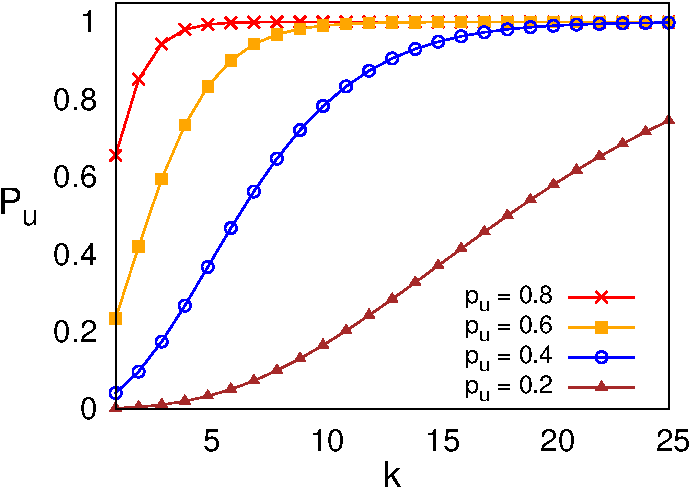
\includegraphics[width=0.45\textwidth]{figures/bdfprs-fig07a} & 
		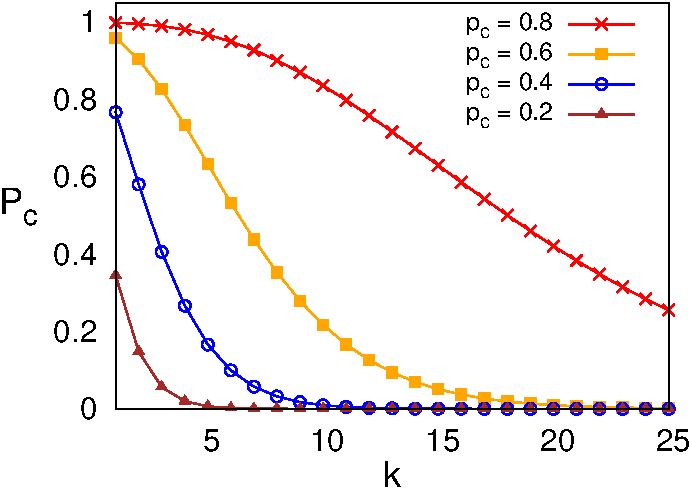
\includegraphics[width=0.45\textwidth]{figures/bdfprs-fig07b} \\[3pt]
		\footnotesize{\hspace{20pt}(a) $\nk=1$,$\ldots,25, \nr=5$} &
		\footnotesize{\hspace{20pt}(b) $\nk=1$,$\ldots,25, \nr=5$} \\[20pt]  
		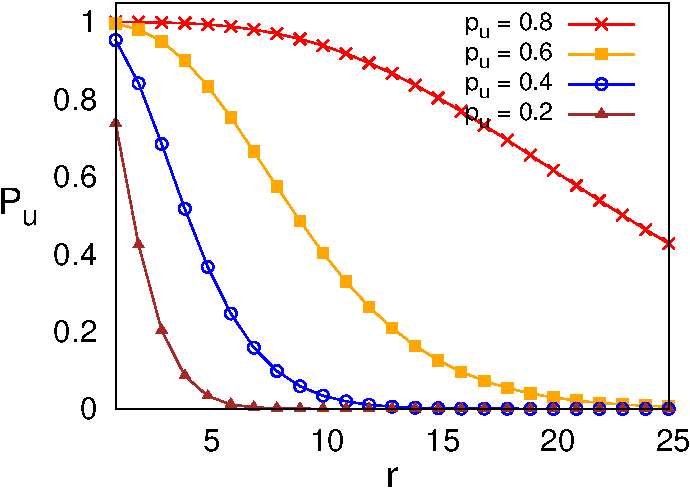
\includegraphics[width=0.45\textwidth]{figures/bdfprs-fig07c} &
		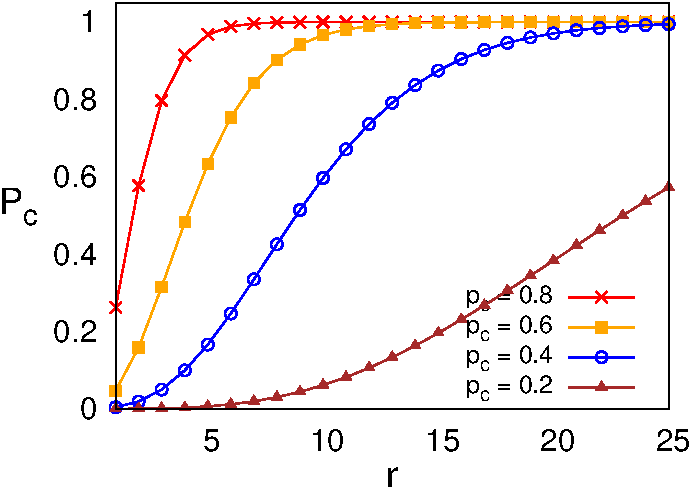
\includegraphics[width=0.45\textwidth]{figures/bdfprs-fig07d} \\[3pt]
		\footnotesize{\hspace{20pt}(c)  $\nk=5$, $\nr=1,\ldots,25$} &
		\footnotesize{\hspace{20pt}(d) $\nk=5$, $\nr=1,\ldots,25$} \\[20pt]
	\end{tabular}
	\caption{\label{dcs:fig:kompact} Probability that the resource is
		unavailable (a,c) and that it is exposed (b,d) using a
		$(\nk,\nr)$-allocation that minimizes the number of nodes, with
		$\nr=5$ varying \nk\ between 1 and 25 (a,b), and with $\nk=5$
		varying \nr\ between 1 and 25 (c,d)}
\end{figure}

\subsection{\compact allocation}\label{dcs:sec:minnode}

Using a $(\nk,\nr)$-allocation with the minimum number of nodes, the
unavailability of the resource occurs when any combination of \nr\ (or
more) nodes becomes unavailable. In fact, regardless of the slices
that those nodes store, such an event causes at least one slice to be
unavailable.  The probability \PF\ that a resource becomes unavailable
is then $\PF= \sum\limits_{i={\R}}^{{\K}+{\R}} {{\K+\R}\choose{i}}
(\pf)^i (1 - \pf)^{{\K}+{\R}-i}$, where the binomial coefficient
${{\K+\R}\choose{i}}$ is the number of all possible combinations of
$i$ nodes over $\nk+\nr$, with $i$ varying in the range
$\nr,\ldots,\nk+\nr$, that can be unavailable; $(\pf)^{i}$ is the
probability that $i$ nodes are unavailable; and $(1 -
\pf)^{{\K}+{\R}-i}$ is the probability that the remaining nodes (i.e.,
$\nk+\nr-i$) are available.  In the same vein, any coalition of
$\nk+1$ nodes causes an exposure of the resource, regardless of the
slices they store. Relying on the minimum number of nodes, in fact,
implies that any coalition of $\nk+1$ nodes possesses all the slices
(Theorem~\ref{dcs:theo:p4}).  The probability \PC\ of a compromise is then
$\PC= \sum\limits_{i={\K}+1}^{{\K}+{\R}} {{\K+\R}\choose{i}} (\pc)^i
(1 - \pc)^{{\K}+{\R}-i}$, where the binomial coefficient
${{\K+\R}\choose{i}}$ is the number of all possible coalitions of $i$
nodes over $\nk+\nr$ nodes, with $i$ varying in the range
$\nk+1,\ldots,\nk+\nr$; $(\pc)^i$ is the probability that $i$ nodes
form a coalition; and $(1 - \pc)^{{\K}+{\R}-i}$ is the probability
that the remaining nodes (i.e., $\nk+\nr-i$) are not compromised.  The
following theorem proves such observations.


\smallskip
\begin{theorem}\label{dcs:teo:security-kompact}
Given a set \Shards\ of slices composing a resource, a set \Nodes\ of
nodes with probability of failure \pf\ and probability of being
compromised \pc, and a $(\nk,\nr)$-allocation using the minimum number
of nodes:
	\begin{align*}
		  & \PF = \sum\limits_{i={\R}}^{{\K}+{\R}} {{\K+\R}\choose{i}} (\pf)^i (1 - \pf)^{{\K}+{\R}-i} \\
		  & \PC = \sum\limits_{i={\K}+1}^{{\K}+{\R}}{{\K+\R}\choose{i}} (\pc)^i (1 - \pc)^{{\K}+{\R}-i}
	\end{align*}
\end{theorem}
\smallskip



Figure~\ref{dcs:fig:kompact} illustrates how \nk\ and \nr\ affect the
values of \PF\ (Figures~\ref{dcs:fig:kompact}(a,c)) and
\PC\ (Figures~\ref{dcs:fig:kompact}(b,d)), considering different values of
\pf\ and \pc, respectively. The values considered for \pf\ and
\pc\ are 0.2, 0.4, 0.6, and 0.8. Figure~\ref{dcs:fig:kompact}(a) reports
the values of \PF\ assuming a fixed number $\nr=5$ of replicas and
varying \nk\ between 1 and 25.  Figure~\ref{dcs:fig:kompact}(c) reports
the values of \PF\ assuming a fixed $\nk=5$ and varying the number
\nr\ of replicas between 1 and 25. Figures~\ref{dcs:fig:kompact}(b,d)
report the values of \PC\ in the same settings as
Figures~\ref{dcs:fig:kompact}(a,c). From the figures, it is immediate to
see that \PF\ and \PC\ present a similar behavior when adopting a
configuration minimizing the number of slices and of nodes (i.e.,
\PF\ increases as \nk\ grows and decreases as \nr\ grows, while
\PC\ decreases as \nk\ grows and increases as \nr\ grows).


\begin{figure}[!t]
	\centering
	\hspace*{-25pt}
	\setlength{\tabcolsep}{20pt}
   \begin{tabular}{cccccc}
	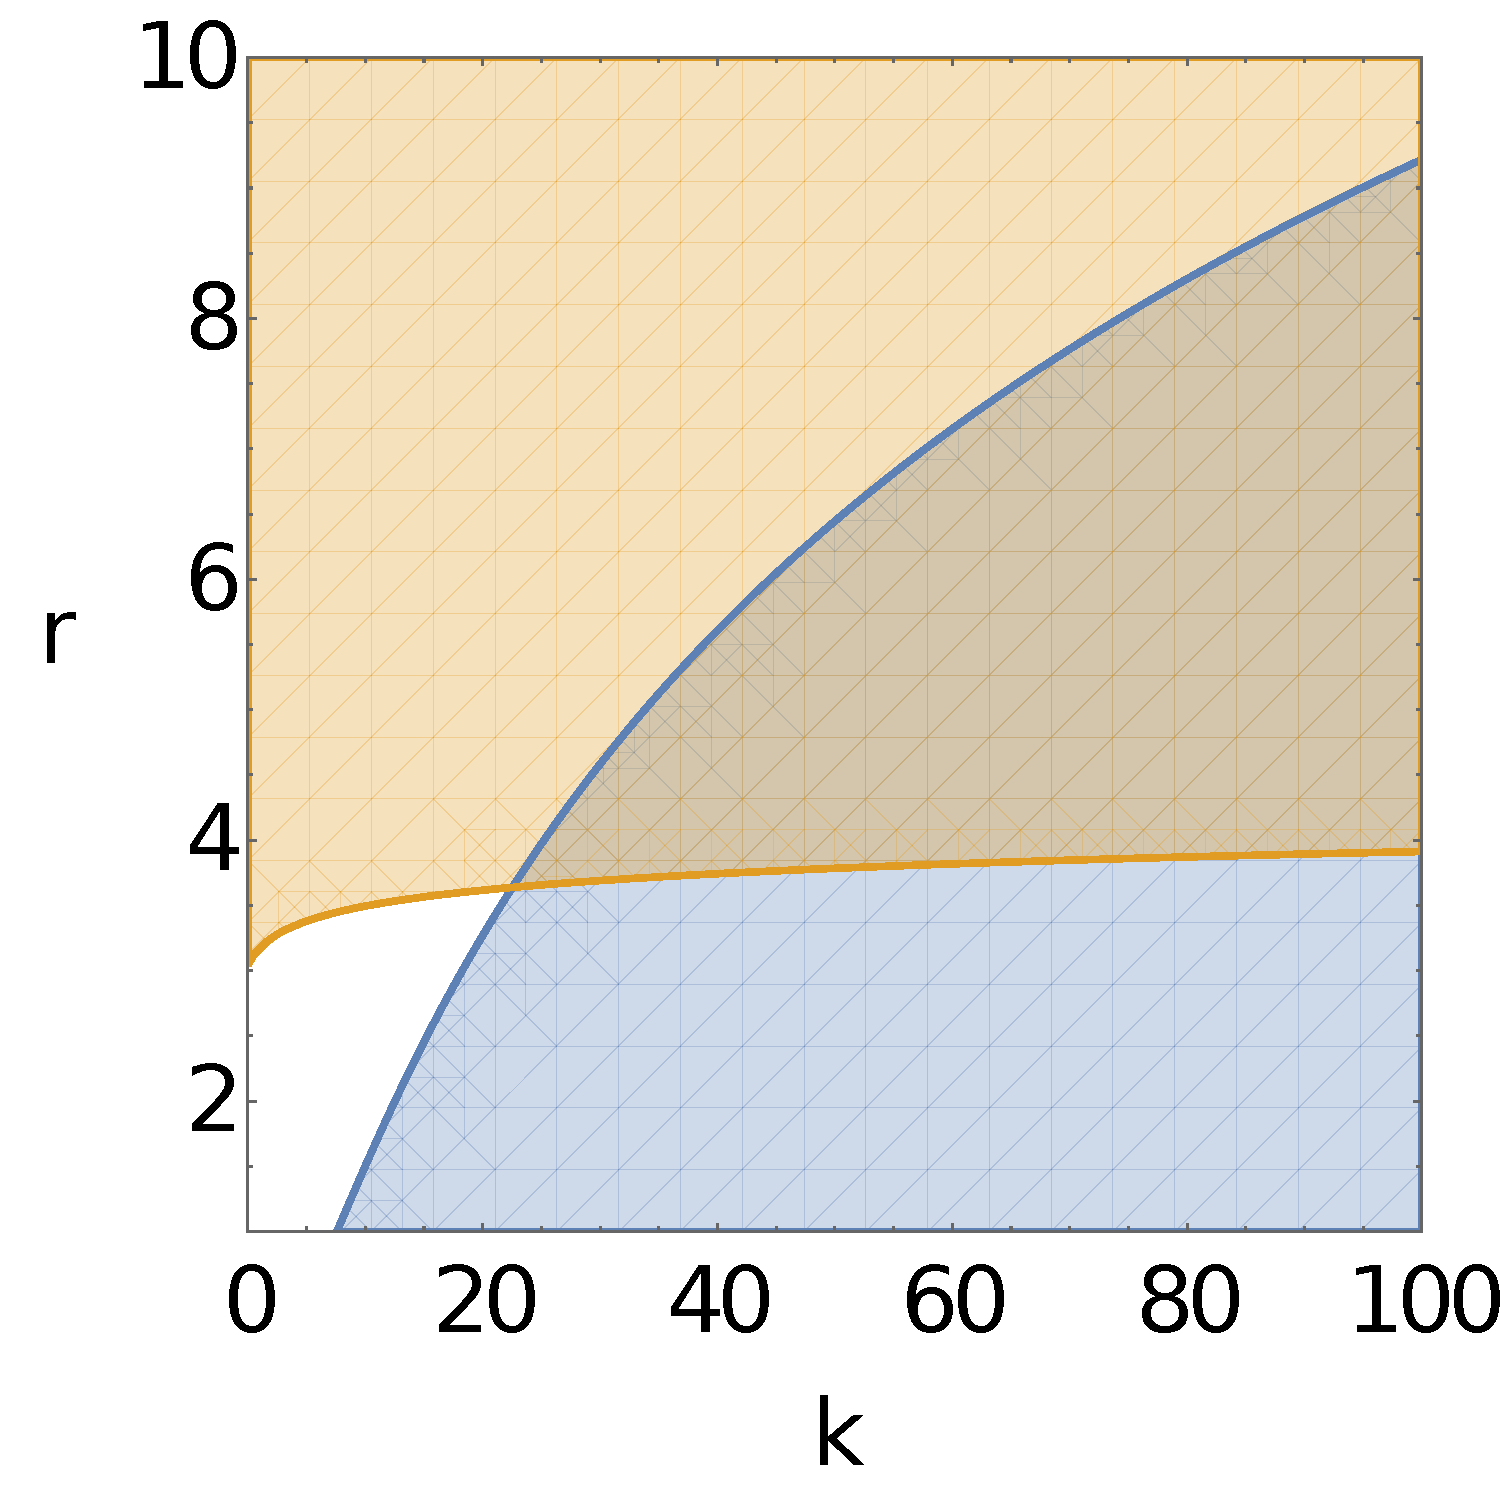
\includegraphics[width=0.33\textwidth]{figures/bdfprs-fig08a} &
	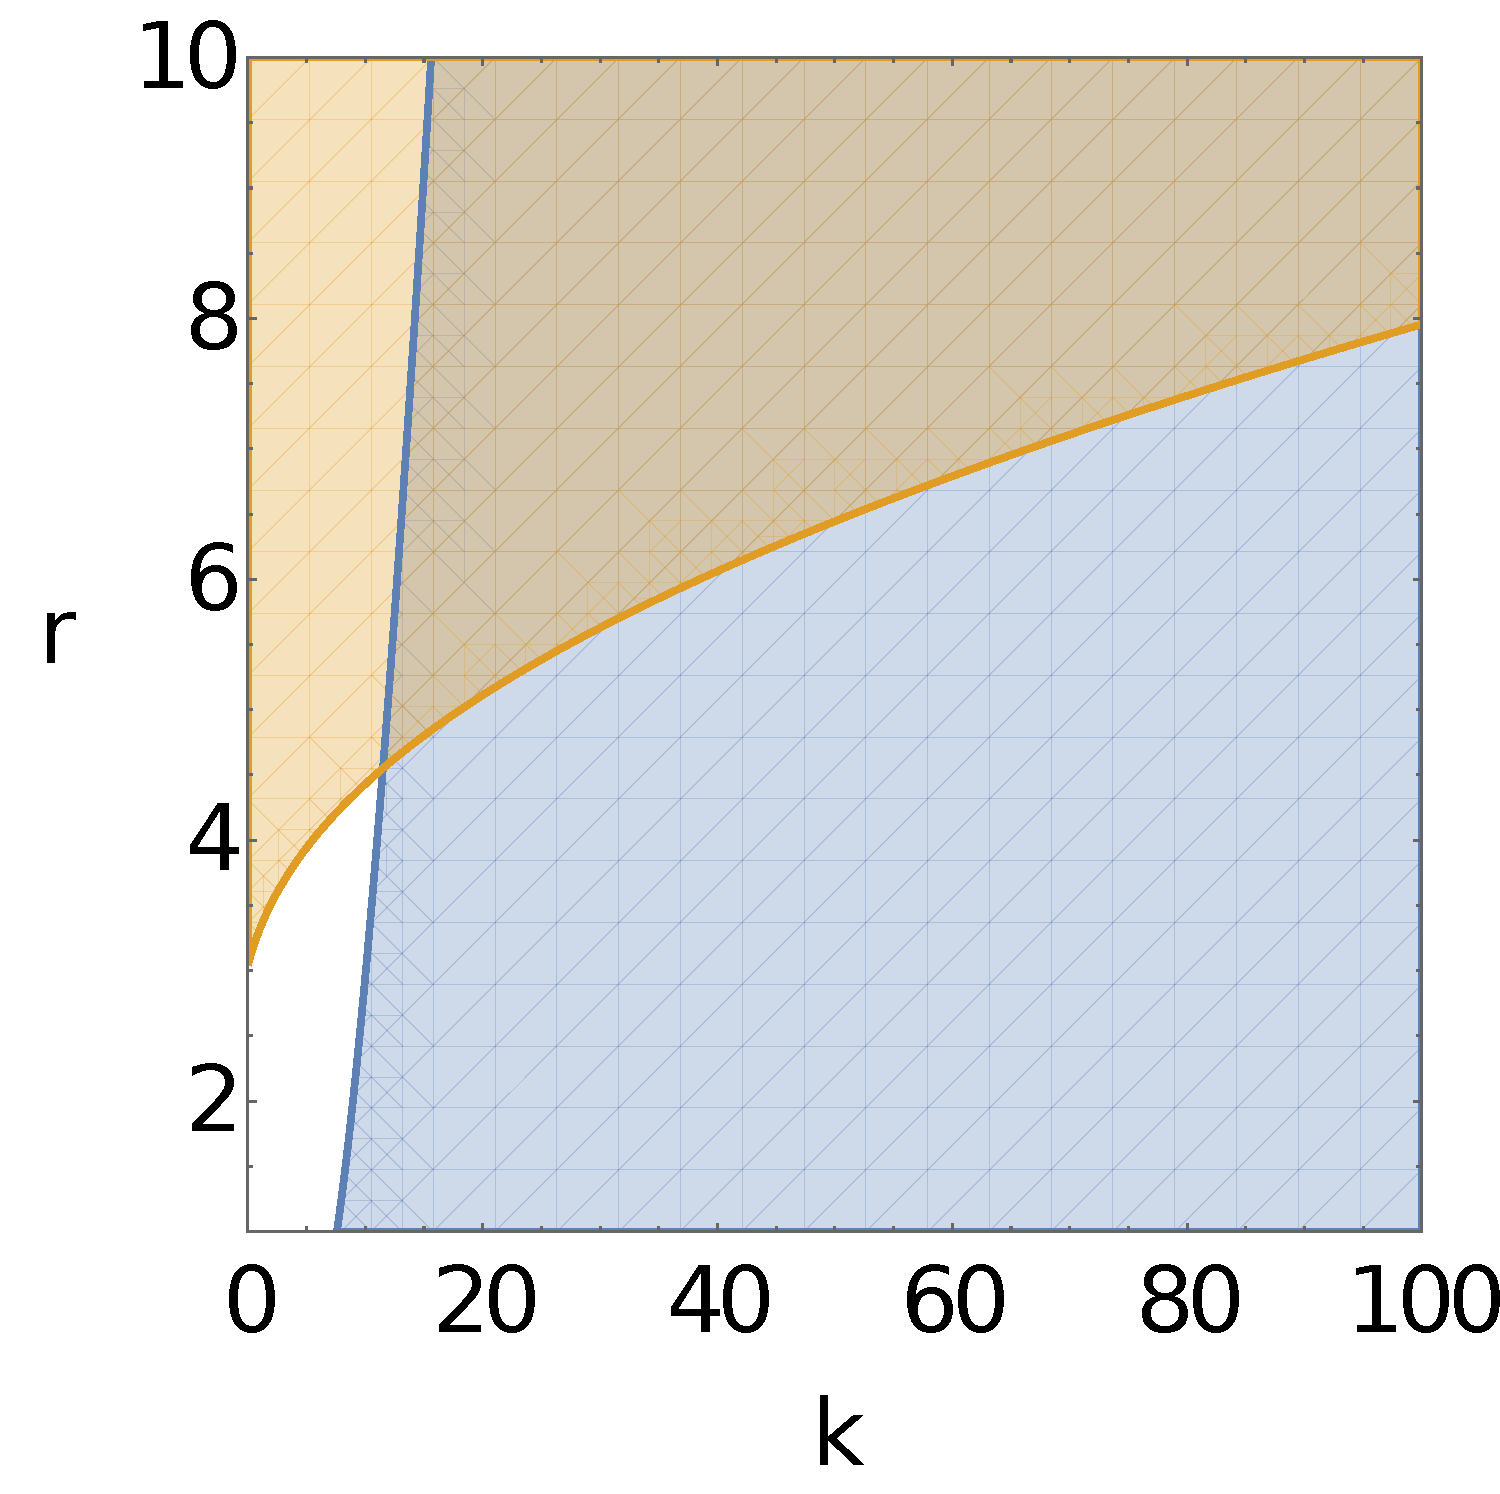
\includegraphics[width=0.33\textwidth]{figures/bdfprs-fig08b} \\[3pt]
	\hspace*{10pt}\shortstack[c]{\footnotesize{(a) \diagonal,} \\ \footnotesize{\pf=0.005, \pc=0.2}} &
	\hspace*{18pt}\shortstack[c]{\footnotesize{(b) \compact,}  \\ \footnotesize{\pf=0.005, \pc=0.2}} \\[20pt]
   	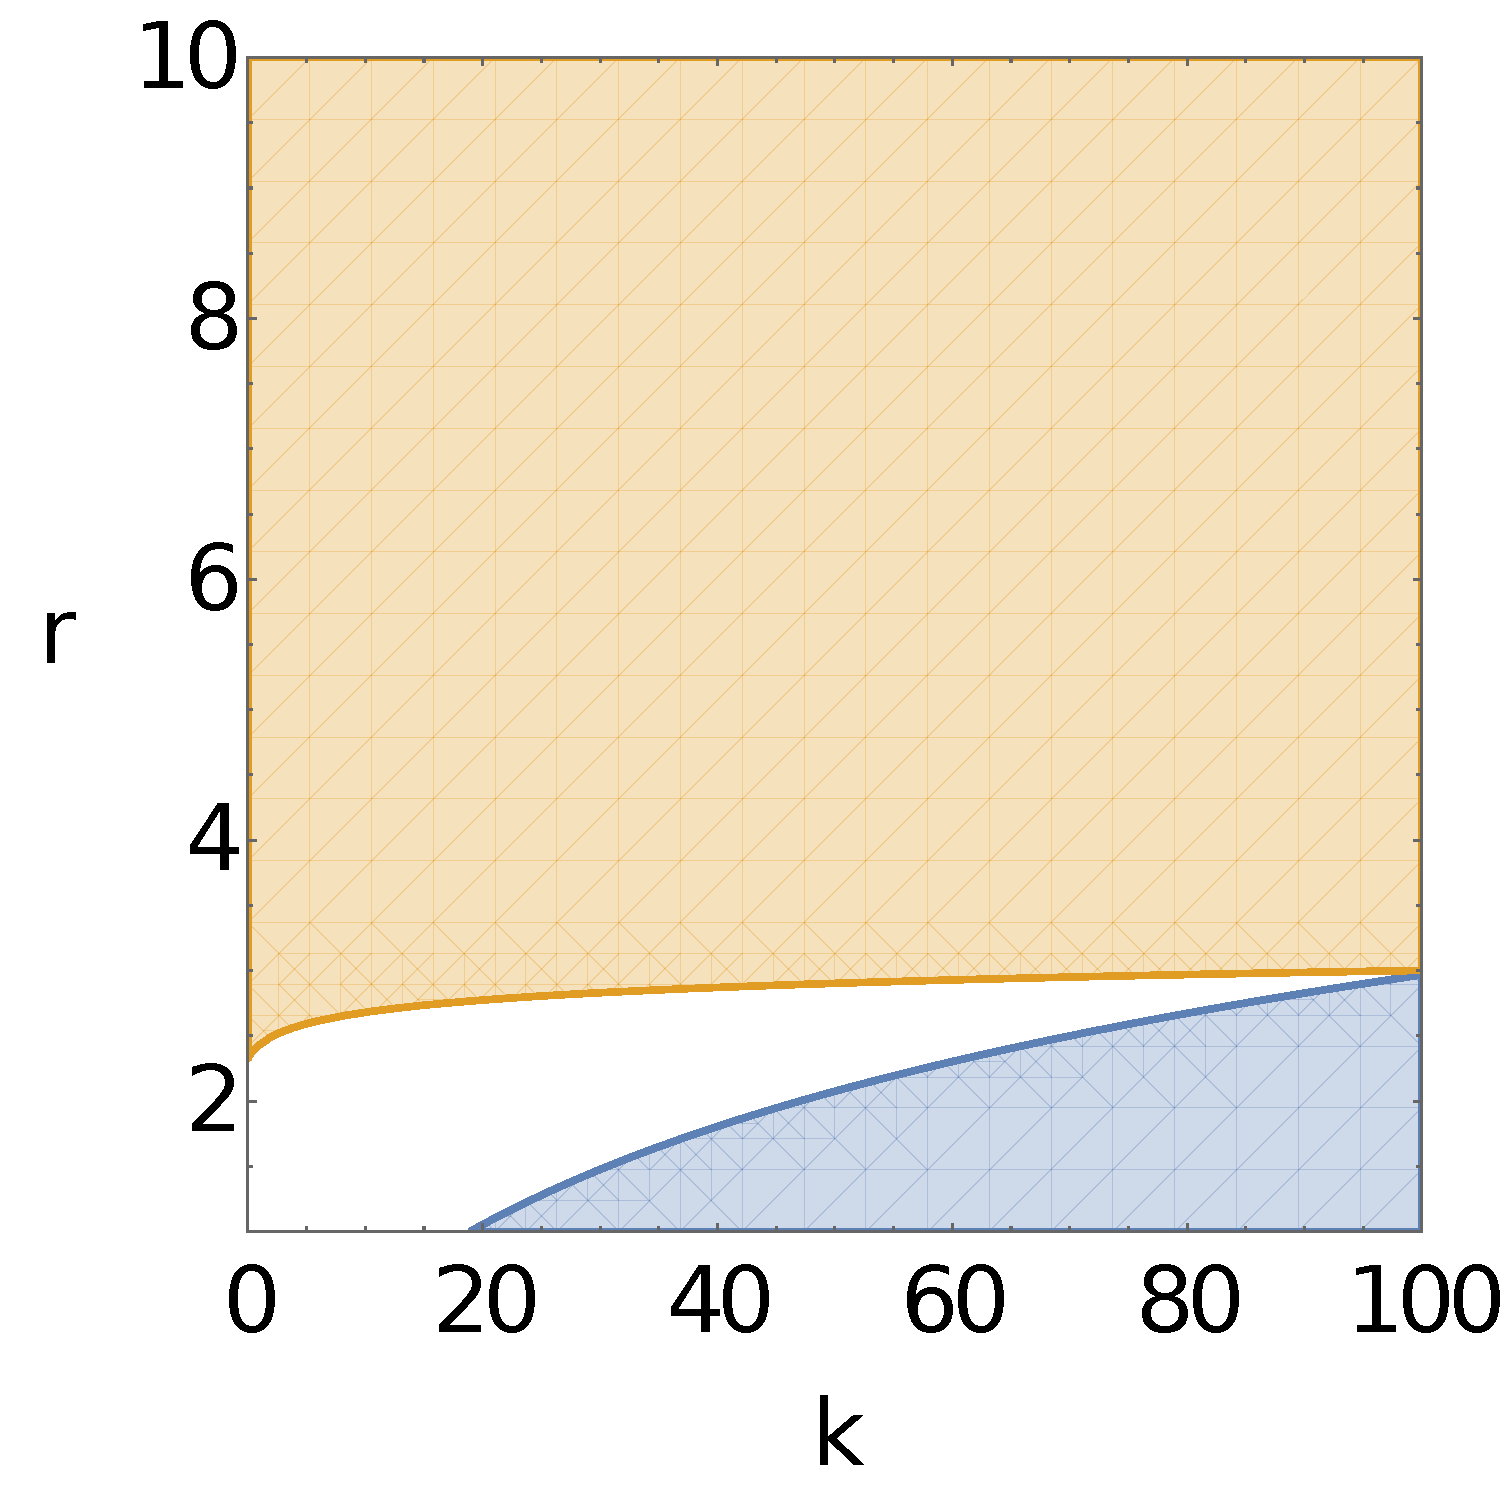
\includegraphics[width=0.33\textwidth]{figures/bdfprs-fig08c} &
   	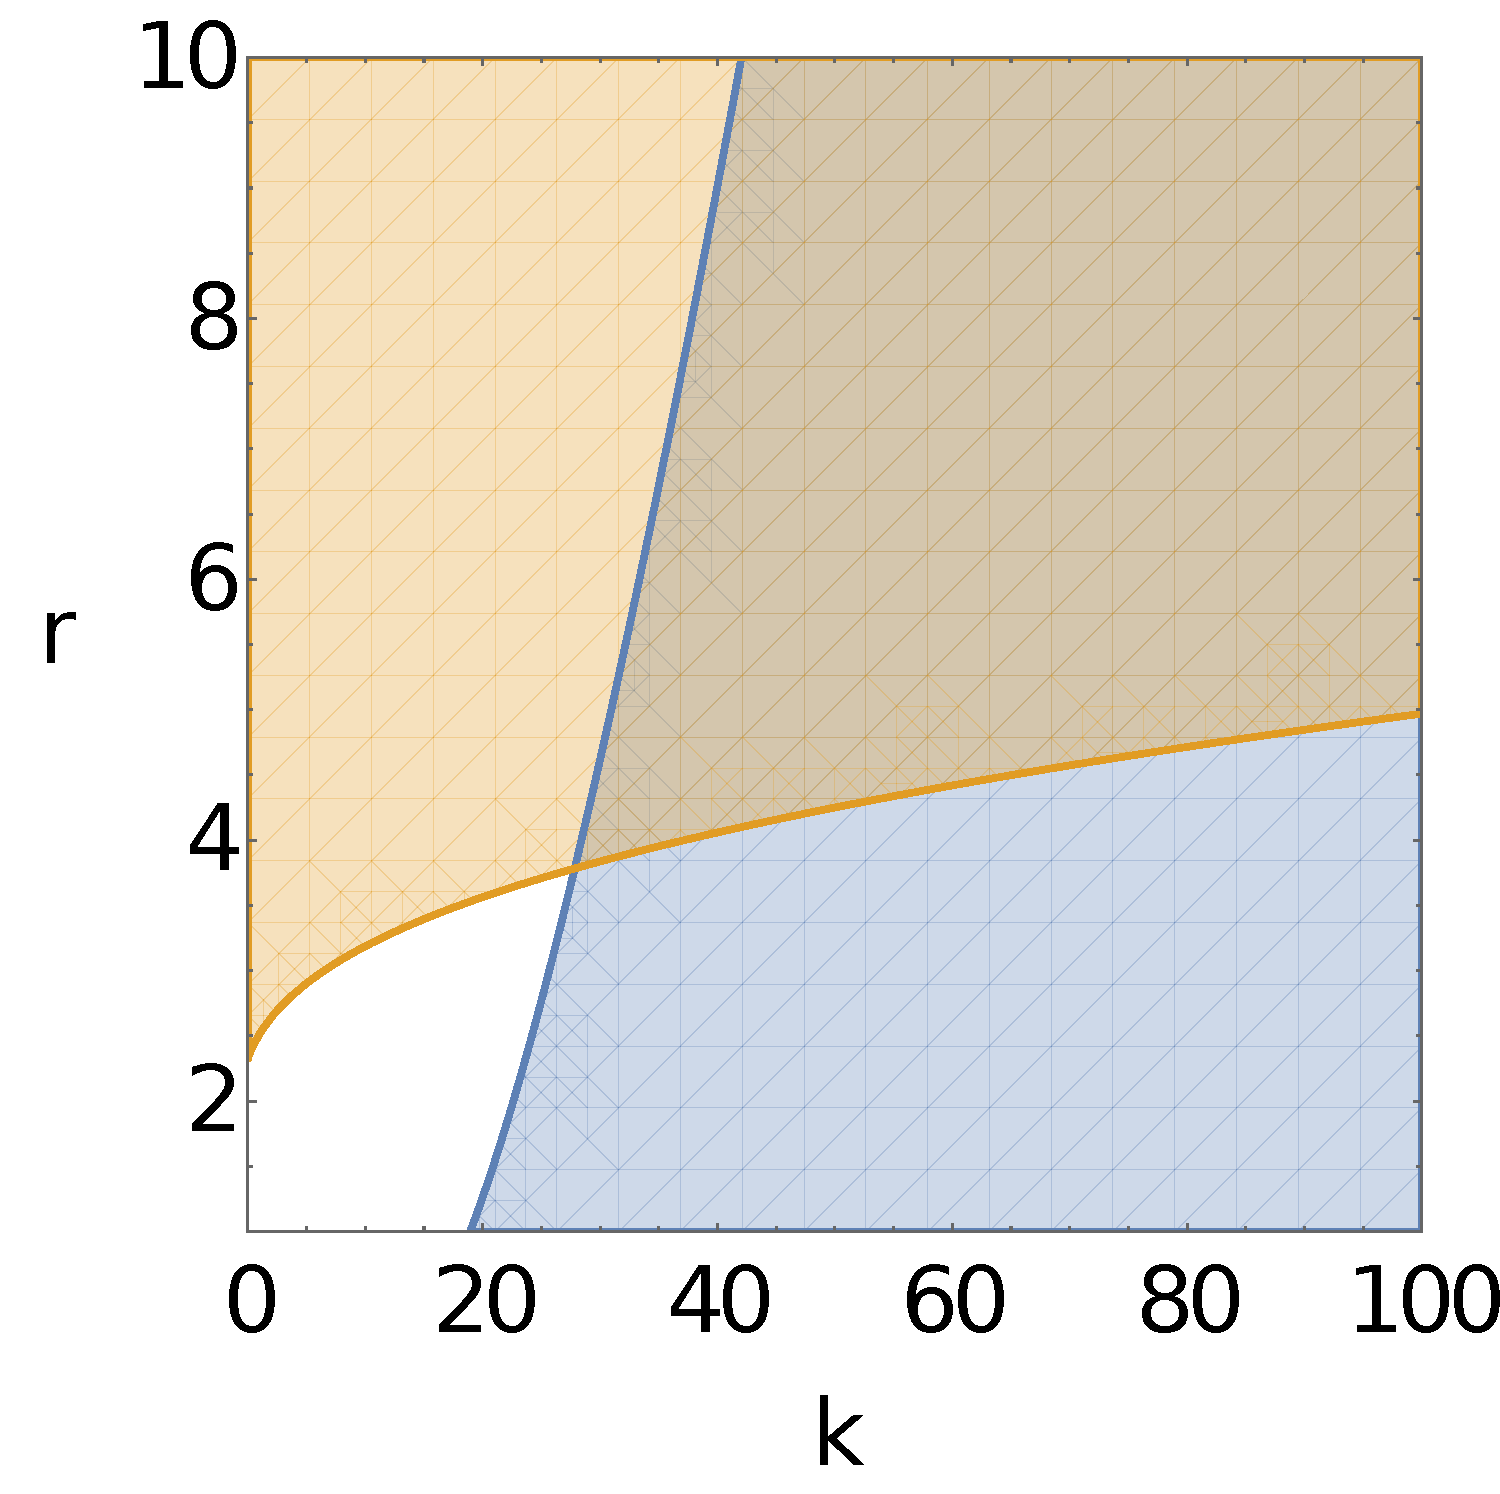
\includegraphics[width=0.33\textwidth]{figures/bdfprs-fig08d} \\[3pt]
	\hspace*{18pt}\shortstack[c]{\footnotesize{(c) \diagonal,} \\ \footnotesize{\pf=0.001, \pc=0.5}} &
	\hspace*{18pt}\shortstack[c]{\footnotesize{(d) \compact,}  \\ \footnotesize{\pf=0.001, \pc=0.5}} \\[20pt]
   	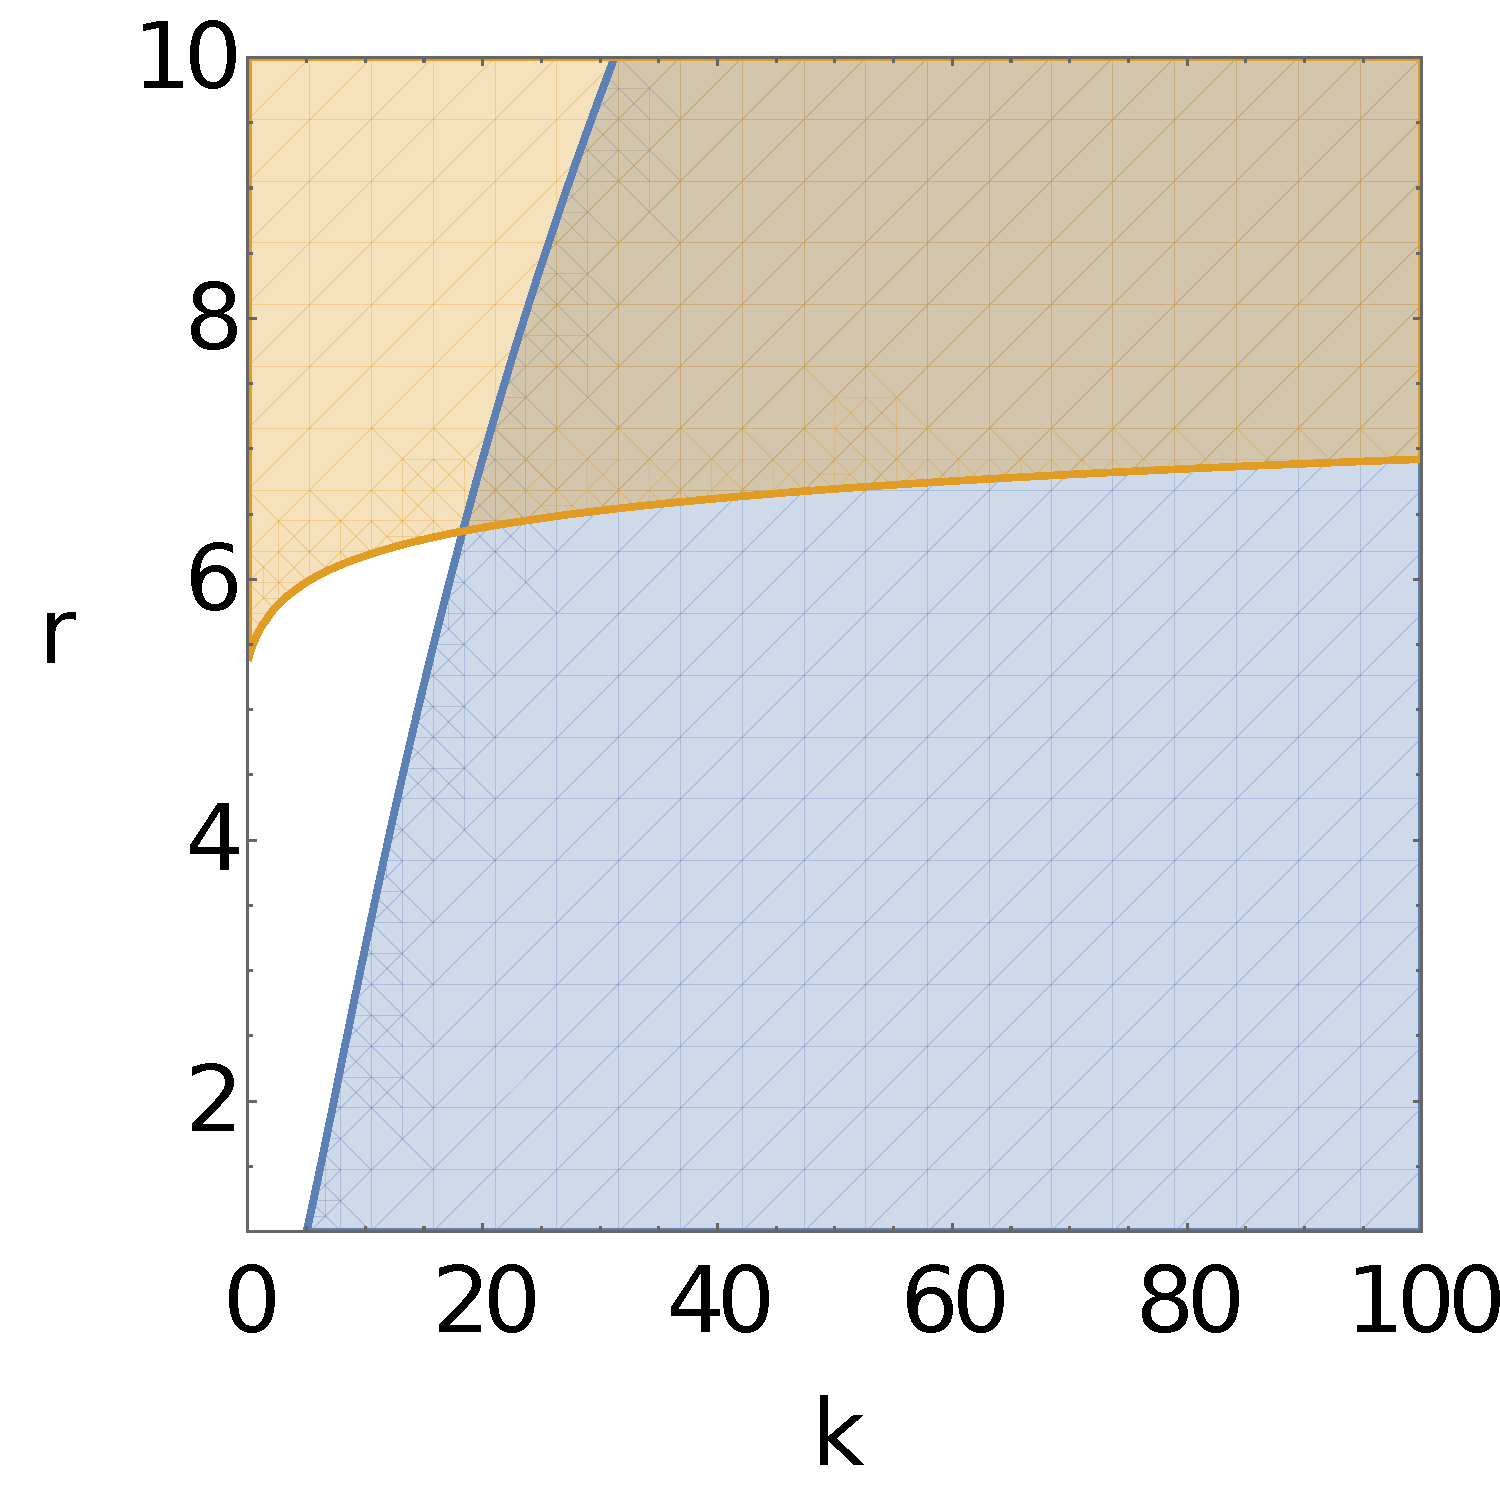
\includegraphics[width=0.33\textwidth]{figures/bdfprs-fig08e} &
   	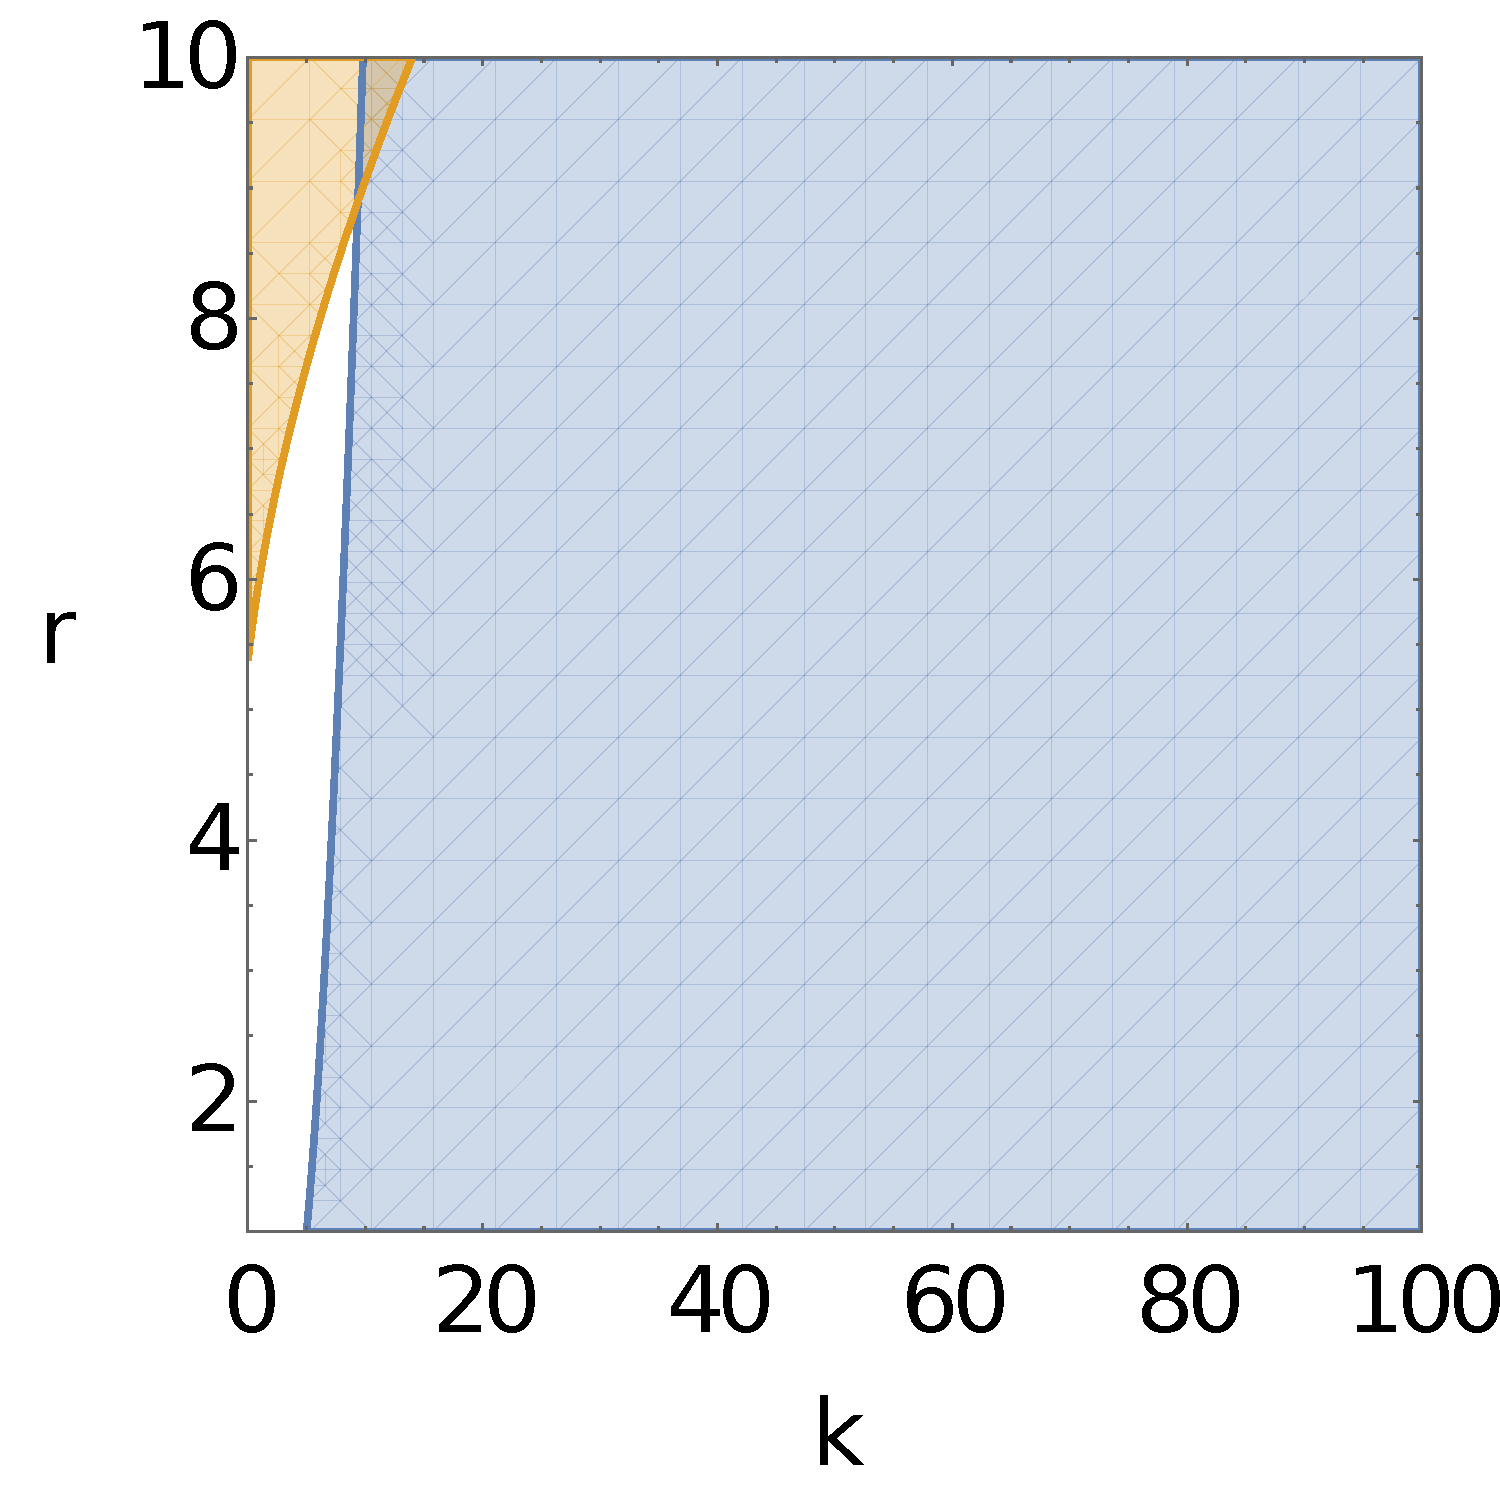
\includegraphics[width=0.33\textwidth]{figures/bdfprs-fig08f} \\[3pt]
	\hspace*{18pt}\shortstack[c]{\footnotesize{(e) \diagonal,} \\ \footnotesize{\pf=0.05, \pc=0.1}}  &
	\hspace*{18pt}\shortstack[c]{\footnotesize{(f) \compact,}  \\ \footnotesize{\pf=0.05, \pc=0.1}} \\[20pt]
   \end{tabular}
   \caption{\label{dcs:fig:compare}\diagonal\ and \compact\ $(\nk,\nr)$-allocations that guarantee $\PF\leq10^{-7}$ and $\PC\leq10^{-6}$ with different values for \pf\ and \pc}
\end{figure}


\subsection{Setting \texorpdfstring{$\boldsymbol{\nk}$}{k} and \texorpdfstring{$\boldsymbol{\nr}$}{r}}\label{dcs:sec:paramenters}

Our modeling of the probability that a resource is not available (\PF)
and that it is exposed (\PC) can be used to set appropriate values for
parameters \nk\ and \nr. To this purpose, fixing the maximum threshold
\PFmax\ of resource unavailability and \PCmax\ of resource exposure,
we compute all the configurations of \nk\ and \nr\ that guarantee $\PF
\leq \PFmax$ and $\PC \leq \PCmax$ through the formulas in
Theorems~\ref{dcs:teo:probability-diagonal}
and~\ref{dcs:teo:security-kompact}. Clearly, the values of \nk\ and
\nr\ for the configurations satisfying the thresholds depend on the
chosen allocation function.


Comparing the evolution of the probability \PF\ that a resource
becomes unavailable using the \diagonal\ and \compact\ allocation
strategies, varying \nk\ (Figure~\ref{dcs:fig:diagonal}(a) and
Figure~\ref{dcs:fig:kompact}(a)), we can easily see that \diagonal\ is
more robust against node failure (i.e., \PF\ increases slowly) than
\compact. This is due to the fact that even if the number of nodes
involved in the allocation increases in both configurations, with an
allocation that minimizes the number of nodes the impact of a node
failure on the availability of the resource is significant. A similar
comment applies when comparing how \PF\ evolves in the two
configurations varying the number \nr\ of replicas
(Figure~\ref{dcs:fig:diagonal}(c) and Figure~\ref{dcs:fig:kompact}(c)). In
this case, the decrease of \PF\ with \diagonal\ is faster than the
decrease of \PF\ with \compact. Therefore, we can conclude that, for
configurations with the same values for \R\ and \K,
\diagonal\ exhibits higher availability.

Comparing the evolution of the probability \PC\ that a resource is
exposed due to a coalition of at least $\nk+1$ nodes using
\diagonal\ and \compact\ allocation strategies, varying
\nk\ (Figure~\ref{dcs:fig:diagonal}(b) and Figure~\ref{dcs:fig:kompact}(b)),
we can easily see that \compact\ is more robust (i.e., \PC\ decreases
faster) than \diagonal. This is due to the fact that, with an
allocation that minimizes the number of nodes, the probability of
forming a coalition of at least $\nk+1$ nodes among the $\nk+\R$ nodes
is smaller than the probability of controlling at least one of the
\R\ nodes for each of the $\nk+1$ slices of the allocation that
minimizes the slices. A similar comment applies when comparing how
\PC\ evolves in the two configurations varying the number of replicas
(Figure~\ref{dcs:fig:diagonal}(d) and Figure~\ref{dcs:fig:kompact}(d)). The
increase of probability \PC\ using \diagonal\ is faster than the
increase of \PC\ using \compact, because it is more difficult to
control at least $\nk+1$ of the $\nk+\R$ nodes than to control at
least one node in each of the distinct $\nk+1$ groups of
\R\ nodes. Therefore, we can conclude that, for configurations with
the same values for \R\ and \K, \compact\ exhibits higher security.


When the resource owner has chosen the preferred allocation function,
given the maximum threshold \PFmax\ of resource unavailability and
\PCmax\ of resource exposure, different configurations of \nk\ and
\nr\ guarantee that $\PF \leq \PFmax$ and $\PC \leq \PCmax$. Among all
these configurations, the ones with low replication factor (\nr)
require less storage and have lower economic costs, while the ones
involving a limited number (\nn) of nodes enjoy simplicity in the
management of the system and better performance of access operations
(less connections have to be established).  Figure~\ref{dcs:fig:compare}
considers three different network configurations, characterized by a
different probability \pf\ for single nodes to fail and a different
probability \pc\ to behave maliciously, and illustrates the
configurations of \nk\ and \nr\ satisfying the above thresholds using
\diagonal\ and \compact\ allocation strategies. In the figure, the
orange area on the top-left represents the configurations of \nk\ and
\nr\ that satisfy the availability requirement (i.e., $\PF \leq
10^{-7}$), while the blue area on the bottom-right represents the
configurations that satisfy the security requirement (i.e., $\PC \leq
10^{-6}$). We chose these thresholds because the overall availability
guarantee ($\PFmax = 10^{-7}$) is the same declared in the
specification of the system used in our experiments (i.e., Storj). We
chose a higher value for $\PCmax$ than $\PFmax$ because protection
against coalitions represents a security layer adding to the
protection already offered by encryption. The intersection between the
orange and blue areas represents configurations that provide both
availability and security guarantees within the thresholds set by the
owner. Among these configurations, the one located on the left/bottom
corner of the intersecting area is the one to be preferred as the
number of nodes and replicas is minimum.


Figures~\ref{dcs:fig:compare}(a,b) consider nodes with $\pf=0.005$ and
$\pc=0.2$. The optimal configuration for \diagonal\ it is $\nk=26$ and
$\nr=4$ (i.e., $\nn=108$), while for \compact\ allocation is $\nk=12$
and $\nr=5$ (i.e., $\nn=17$). The second allocation, although more
expensive on storage, due to one additional replica, considerably
reduces the number of nodes involved in the storage of the resource
compared to the adoption of the first allocation function. Our
analysis demonstrates that this is a general behavior:
\compact\ requires the same (or a slightly higher) number \R\ of
replicas and a significantly lower number \N\ of nodes than
\diagonal. This observation is confirmed by the extreme scenarios
illustrated in Figures~\ref{dcs:fig:compare}(c,d), considering highly
reliable ($\pf = 0.001$) but lowly trusted ($\pc = 0.5$) nodes, and in
Figures~\ref{dcs:fig:compare}(e,f), considering unreliable ($\pf = 0.05$)
but relatively trusted ($\pc = 0.1$) nodes.  The optimal
configurations in Figures~\ref{dcs:fig:compare}(c,d) are $\nk=100$ and
$\nr=3$ for \diagonal\ (i.e., $\nn=303$), and $\nk=27$ and $\nr=4$ for
\compact\ (i.e., $\nn=31$, meaning that the number of nodes is ten
times smaller). The optimal configurations in
Figures~\ref{dcs:fig:compare}(e,f) are $\nk=10$ and $\nr=9$ (i.e.,
$\nn=99$) for \diagonal, and $\nk=18$ and $\nr=7$ (i.e., $\nn=25$) for
\compact.


Our analysis confirms that, for a wide range of values
for \PF\ and \PC\ and assumptions on the node availability \pf\ and
compromise risk \pc, our approach is able to identify a configuration
of \R\ and \K\ with  manageable complexity (i.e., a reasonable number of replicas and of nodes). We note that, even when
\R\ and \K\ grow, the minimum number of slices composing a resource remains
limited. 




\section[Experiments]{Implementation and Experiments}\label{dcs:sect:implementation}
To verify the benefit of our proposal we applied it into an existing
DCS network. Among the existing DCS networks (e.g., {\em
  Storj}~\cite{wilkinson2014storj}, {\em Sia}~\cite{vorick2014sia},
{\em IPFS}~\cite{benet2014ipfs}, and {\em Maidsafe
  Safe-network}~\cite{lambert2014safenetwork}), we selected Storj
since, to the best of our knowledge, it is currently the most advanced
and supported DCS.  The market valuation of the
cryptocurrencies~\cite{cslr18} associated with these DCSs (Storj for
Storj, Siacoin for Sia, Filecoin for IPFS, and Maidsafecoin for
Maidsafe) supports the importance that these solutions are rising: at
the date of submission, the global market capitalization of these
initiatives is more than 400 million dollars.  There are currently
more than 100,000 nodes offering capacity in the Storj network, with
more than 100PB of data available and a planned goal of 10 times
growth in 2019.

Storj is a protocol that coordinates a decentralized network to create
and enforce storage contracts between peers. Each peer can negotiate
contracts with other peers, upload and download data from other peers,
and periodically verify the availability and integrity of her data.
Storj leverages a Distributed Hash Table (DHT) to connect parties
interested in forming a storage contract.  In the discussion, we
maintain the terminology of our model and refer to parties outsourcing
their resources to the decentralized network as owners ({\em
  renters\/} in Storj), and to parties offering storage space in
exchange for a remuneration in a digital currency as storage nodes
({\em farmers\/} in Storj).  {\em Bridge nodes\/} support the correct
operations in the system and can take responsibility for the
verification of the integrity and availability of resources. In the
following, we describe the technical choices characterizing our
implementation (Section~\ref{dcs:ss:implementation}), the experimental
results (Section~\ref{dcs:ss:results}), and a few considerations about the
impact produced by fine granularity retrieval (Section~\ref{dcs:ss:further}).
    

\subsection{Implementation}\label{dcs:ss:implementation}
The enforcement of \diagonal\ and \compact\ allocation strategies in
Storj required changing the client library of the open source
implementation.  In particular, Storj currently offers three main
clients, one written in C that must be built from source, one written
in JavaScript and designed to be executed by a node.js runtime, and
one written in Python and compatible with any Python environment. We
integrated our technique within the Python implementation, also for
easy integration with the implementation of \name, which in addition
of being an AONT-encryption supports other protection requirements
(e.g., encryption-based access control and policy revocation).  The
design of Storj makes the client independent from the bridge and the
storage nodes. Our work on the Python client allowed us to access the
services of the whole network.

We implemented the \diagonal\ and \compact\ allocation strategies in
the client and assigned slices (in the Storj terminology all the
slices allocated to a node form a {\em shard\/}) to nodes. The
performance of shard creation and resource reconstruction is orders of
magnitude greater than the throughput of storage nodes in the Storj
network (\name\ operates at several hundred MB/s, whereas the maximum
throughput we observed in Storj is around two orders of magnitude
lower). In our experiments, we focused on evaluating the time required
to complete the access request since the time requested by decryption
does not have significant impact.  We note that the use of the AONT
forces each access request to be able to proceed with a client-side
decryption only when the complete resource is available on the client.
Should this be a problem for the specific application domain (e.g.,
resources are very large), mitigation can be provided by splitting the
large resource and applying our approach to the resulting (smaller)
chunks. Each chunk can then be downloaded and decrypted
independently. This would reduce the access times to resources, but it
may also delay the completion of the transfer, because the overhead
for the management of a greater number of access requests reduces the
effective bandwidth. The experiments confirm this observation (see
Section~\ref{dcs:ss:results}), as they show that there is a performance
benefit in managing large resources.


\subsection{Experimental results}\label{dcs:ss:results}
To evaluate the performance of the \diagonal\ and \compact\ allocation
strategies, we introduced into the client a module that activates a
number of parallel threads (in the considered configuration, we used
10 concurrent threads) to open access requests to the storage
nodes. In Storj, access requests from the owner involve both storage
nodes and bridge nodes. In fact, each time an owner needs to retrieve
a shard, she makes a request to the bridge, which returns a token
together with the IP address of the node storing the required shard
(note that this access request is recorded and a crypto-currency
payment is created by the owner for the node). The token is then used
by the client as a parameter of an HTTP request directed to the node.
Our experiments considered the performance of the system in the
management of the dialogue between owner and node. In particular, we
compared the access times observed for the two allocation strategies,
varying the resource size.

An important restriction of the current implementation of Storj is
that requests for shards are atomic and it is not possible to access
only a specific portion of a shard managed by a node. This restriction
cannot be removed operating only on the client, as it has a great
impact not only on storage nodes but on the overall structure of the
system.  We then implemented the access requests for the
\diagonal\ and \compact\ techniques as follows.  For \compact, we
implemented concurrent requests to the nodes. As soon as a node
completes the delivery of its shard, a new request is started for
another shard. The request is considered completed as soon as the
client has received $\K+1$ complete shards. For \diagonal, for each
shard a number $t$ of parallel threads ($t \leq \R$) are activated to
manage a request to distinct nodes managing the same shard (which
coincides with a slice for this allocation strategy), for a number of
shards compatible with the number of concurrent threads (e.g., in the
experiments we set $t=2$ and we had 5 shards processed at the same
time by the 10 threads). As soon as a shard is fully delivered to the
client, the group of $t$ threads is dedicated to another missing
shard.

\begin{figure}[!t]
	\centering
	\hspace*{-8pt}
       \begin{tabular}{cc} 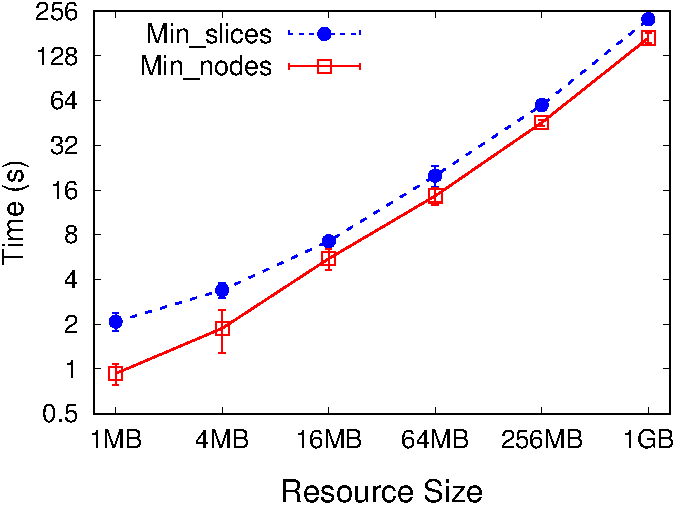
\includegraphics[width=0.475\columnwidth]{./figures/bdfprs-fig09a} &
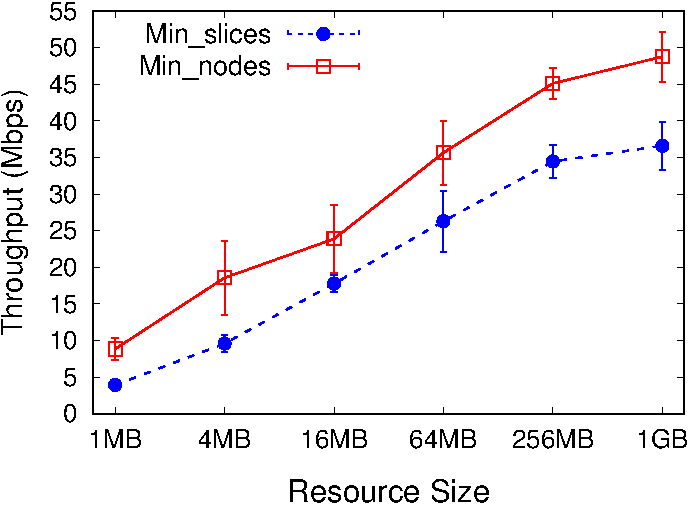
\includegraphics[width=0.475\columnwidth]{./figures/bdfprs-fig09b}\\[-3pt]
           \footnotesize{\hspace*{16pt}(a)} & \footnotesize{\hspace*{16pt}(b)}\\
       \end{tabular}
   \caption{\label{dcs:fig:exp1}Completion time (a) and overall throughput (b)
   in the \diagonal\ and \compact\ allocation strategies}
\end{figure}


Figure~\ref{dcs:fig:exp1} reports the results of our experiments, where we
used resources of size varying from 1MB to 1GB.
Figure~\ref{dcs:fig:exp1}(a) shows the time required for the completion of
the access requests and Figure~\ref{dcs:fig:exp1}(b) shows the throughput
in terms of bandwidth. The graphs include two curves, one for
\diagonal\ allocation, with $\nk=26$ and $\nr=4$, and one for
\compact\ allocation, with $\nk=12$ and $\nr=5$, which correspond to
the configurations considered in Figure~\ref{dcs:fig:compare}(a) and
Figure \ref{dcs:fig:compare}(b), respectively.  The graphs present the
average and the standard deviation of the values obtained with 10
executions. We note that the \compact\ strategy exhibits a moderate
benefit compared to the \diagonal\ strategy. The benefit derives from
the savings in overhead associated with the interaction with multiple
nodes. An element that also contributes to the throughput is the
natural variety of performance in nodes, with some being faster than
others.  The \compact\ strategy works well as long as the number of
nodes with limited performance ({\em slow} nodes) is less than $\nr
-1$ and there are at least $\nk +1$ nodes with good performance ({\em
  fast} nodes) serving the shard. For \diagonal, it is sufficient to
have one of the $\K+1$ shards assigned to a group of nodes where the
$t$ nodes contacted in parallel happen to be slow to suffer from a
significant delay in the access.


\subsection{Further considerations \label{dcs:ss:further}}
 We noted that a limitation of the current implementation of the Storj
 node is that the request for a shard is atomic. The realization of a
 mechanism that permits to manage partial access requests would offer
 the opportunity for a significant improvement in the management of
 the access requests. For a generic server in a file sharing protocol
 this can be expected to be a relatively simple change in the server
 code; for a DCS system, this change would require a revision of the
 model used for the remuneration of access requests, as follows.  The
 bridge should not consider each request received by the owner as an
 access to the complete resource (which also implies a payment to
 access the whole resource), but it should return to the owner the IP
 address and the authorization token of the node storing the
 shard. The owner and the node should then commence a protocol in
 which the owner issues signed confirmations in exchange of pieces of
 the resource. These confirmations can then be submitted to the bridge
 to receive the payment.  Allowing the owner to pay a node only for
 the downloaded portion of the resource results in better performance
 and stronger competition among the nodes; best performing nodes would
 be preferred by the owner and would serve more traffic, receiving a
 correspondingly greater remuneration for their storage service.
 
  The flexible structure of the \compact\ assignment would be
  particularly suited to this model. Under the assumption that nodes
  exhibit a high variability in access times, each slice could be
  retrieved by any of the \R\ nodes storing it, with the possibility
  to adapt the amount of data transferred from each node depending on
  the response time and in case a group of \R\ nodes happens to be all
  composed of slow nodes, the impact would be limited to the single or
  few slices that cannot be retrieved from fast nodes.



\section{Related Work}\label{dcs:sec:relwork}


{\em RAID}~\cite{Patterson:1988:CRA:971701.50214} is one of the main
contributions aimed at the construction of reliable systems.  RAID is
normally deployed on local drives.  With the advent of the cloud, RAID
has been extended to take adversarial failures into
consideration. Along this line of works, {\em HAIL (High-Availability
  and Integrity Layer)}~\cite{bowers2009hail} extended RAID with
multiple cloud storage providers and a {\em Proof of Retrievability
  (PoR)}~\cite{bowers2009proofs} scheme to verify that a provider
still holds a certain piece of information.  {\em HAIL} is however not
well-suited for DCS systems, where the nodes are less reliable than
well-established cloud service providers. Also, {\em HAIL} does not
take into account the possibility of adversarial users trying to
reconstruct the resources for their own personal profit.  The works
closest to ours are the solutions aimed to offer reliability and
security of data in DCS. Many DCS networks that have recently been
proposed, already include a certain degree of security guarantees.
(i.e., protection against malicious parties jointly collecting all the
slices composing a resource).  Among them,
Storj~\cite{wilkinson2014storj} and Sia~\cite{vorick2014sia} adopt
client-side encryption and do not protect the outsourced data against
coalitions of malicious nodes.  SAFE Network~\cite{irvine2010maidsafe}
instead adopts a self-encryption technique: the resource is divided
into shards and a weak AONT among 3 shards is applied before uploading
them.  In~\cite{paul2014security} the design of the SAFE Network and
the possible attack vectors are analyzed.  The solution proposed
in~\cite{irvine2010maidsafe,paul2014security} is predetermined and the
interaction between redundancy and security is not analyzed.  Our
proposal could be applied to improve the flexibility and security of
these networks.


Another line of works is security of outsourced data
(e.g.,~\cite{ajjp16,atl2005,nal14,tppg13}), which can be improved
using AONT. Existing solutions however consider domains different from
DCS. We have discussed before the proposal in~\cite{bdfprs-ccs2016},
where the goal was to support policy evolution for outsourced
resources where the access control policy is mapped to an encryption
policy.  Another approach using AONT and Reed-Solomon codes is
AONT-RS~\cite{rp11aont}.  Apart from the use of AONT, there is a
limited similarity with the structure of our proposal. In fact, the
work in~\cite{rp11aont} does not explicitly consider the structure of
current DCS systems and does not provide an approach for the
identification of the parameters to use in the configuration of the
system.  An evolution of the work on AONT-RS is
CAONT-RS~\cite{li2014convergent} that has been used by
CDStore~\cite{usenixcdstore}, which also uses two-stage deduplication
to achieve both bandwidth and storage savings and robustness against
side-channel attacks, while DepSky~\cite{bessani2013depsky} addresses
the privacy requirements using Shamir's scheme.  All these proposals
consider cloud-of-clouds environments, which see the integration of
the services of cloud providers. Their adaptation to the DCS scenario
requires significant attention and a model for the identification of
the parameters to use in the configuration of the system. Also, the
interaction between security and availability is not analyzed.

A precursor of DCS is represented by P2P systems. The P2P system
closer to our proposal, which considers reliability and security, is
Tangler~\cite{waldman2001tangler}. The goal of Tangler is censorship
resistance, which is a potential application of DCS, but not its main
goal. Several of the assumptions at the basis of the design of Tangler
have also been considered in the realization of DCS systems. A crucial
difference between Tangler and our proposal is that Tangler uses
Shamir's method, so it is quite expensive in terms of storage and
bandwidth. Also, it does not aim at combining availability and
confidentiality requirements in data allocation.

The novelty of our approach with respect to all above-mentioned
techniques is the combination of AONT with different strategies for
slicing and allocating resources in DCS systems and the joint
consideration of security and availability guarantees. Our analysis of
the characterization, interplay, and settings of the parameters
guiding slicing and allocation can be used by all existing solutions
to enhance their security and availability properties.




\section{Conclusions}\label{dcs:sec:conclusion}

We presented an approach for providing effective secure protection to
resources in decentralized cloud storage services.  Our approach
enables resource owners to protect their resources and to control
their decentralized allocation to different nodes in the network. We
investigated different strategies for splitting and distributing
resources, analyzing their characteristics in terms of availability
and security guarantees. We also provided a modeling of the problem
enabling owners to control the granularity of slicing and
diversification of allocation to ensure aimed availability and
security guarantees. Enabling effective control for resource owners,
our solution helps in removing natural reluctance due to security
concerns and moves a step forward in the realization of novel services
effectively benefiting from technological evolution. Our work
  leaves room for extensions, such as the consideration of error
  correcting codes and information dispersal algorithms to reduce the
  spatial overhead.
